This section presents the results of the verification studies used to assess the numerical accuracy and convergence behavior of the computational model. The analysis begins with code verification, where numerical solutions are compared against analytical benchmarks for steady fluid flow, steady heat conduction, and transient thermal diffusion. This is followed by solution verification studies, including both steady-state and transient configurations, to quantify discretization error arising from spatial and temporal resolution, as well as solver tolerance. Together, these results provide evidence of numerical correctness, convergence, and overall model credibility.

\subsection{Code Verification}
Code verification is performed to assess the correctness of the numerical implementation through comparison with analytical solutions. Three problems are considered to independently verify the fluid and thermal components of the \texttt{chtMultiRegionFoam} solver \cite{chtMultiRegion}: Hagen--Poiseuille flow for laminar momentum transport \cite{hagenPoisueille}, steady-state radial conduction with internal heat generation, and transient thermal diffusion using a separation-of-variables Bessel-function solution. The transient diffusion configuration additionally verifies the transient thermal coupling behavior at the fluid-solid interface by ensuring that the imposed solid temperature response is accurately transferred into the fluid region. Although the full conjugate heat transfer solver is used, the configurations are constructed to isolate momentum transport in the fluid, steady conduction in the solid, and transient diffusion in the fluid, respectively. This approach enables rigorous verification of each governing equation prior to evaluating the fully coupled system under solution verification.

\subsubsection{Hydrodynamic (Fluid Only) Model}
To verify the momentum transport implementation, a steady-state laminar pipe flow simulation was compared against the analytical Hagen-Poiseuille solution. Spatial convergence was assessed using four progressively refined meshes with representative cell sizes of 0.43~mm, 0.22~mm, 0.11~mm, and 0.088~mm while maintaining identical geometry and boundary conditions. Axial velocity was evaluated at a cross-sectional plane located beyond the hydrodynamic entry length to ensure fully developed flow. The numerical velocity field was compared pointwise with the analytical solution (Eq.~\ref{eq:poiseuille}).
Figure~\ref{fig:scatterVelocity} shows that the numerical solution progressively aligns with the analytical parabolic profile as mesh resolution improves for three resolutions: coarse (0.43~mm), medium (0.22~mm), and fine (0.11~mm). The coarse mesh overpredicts velocity near the centerline due to insufficient spatial resolution, while refinement at the finest mesh achieves the best agreement.

\begin{figure}[htbp!]
  \centering
  \begin{subfigure}[b]{0.5\textwidth}
    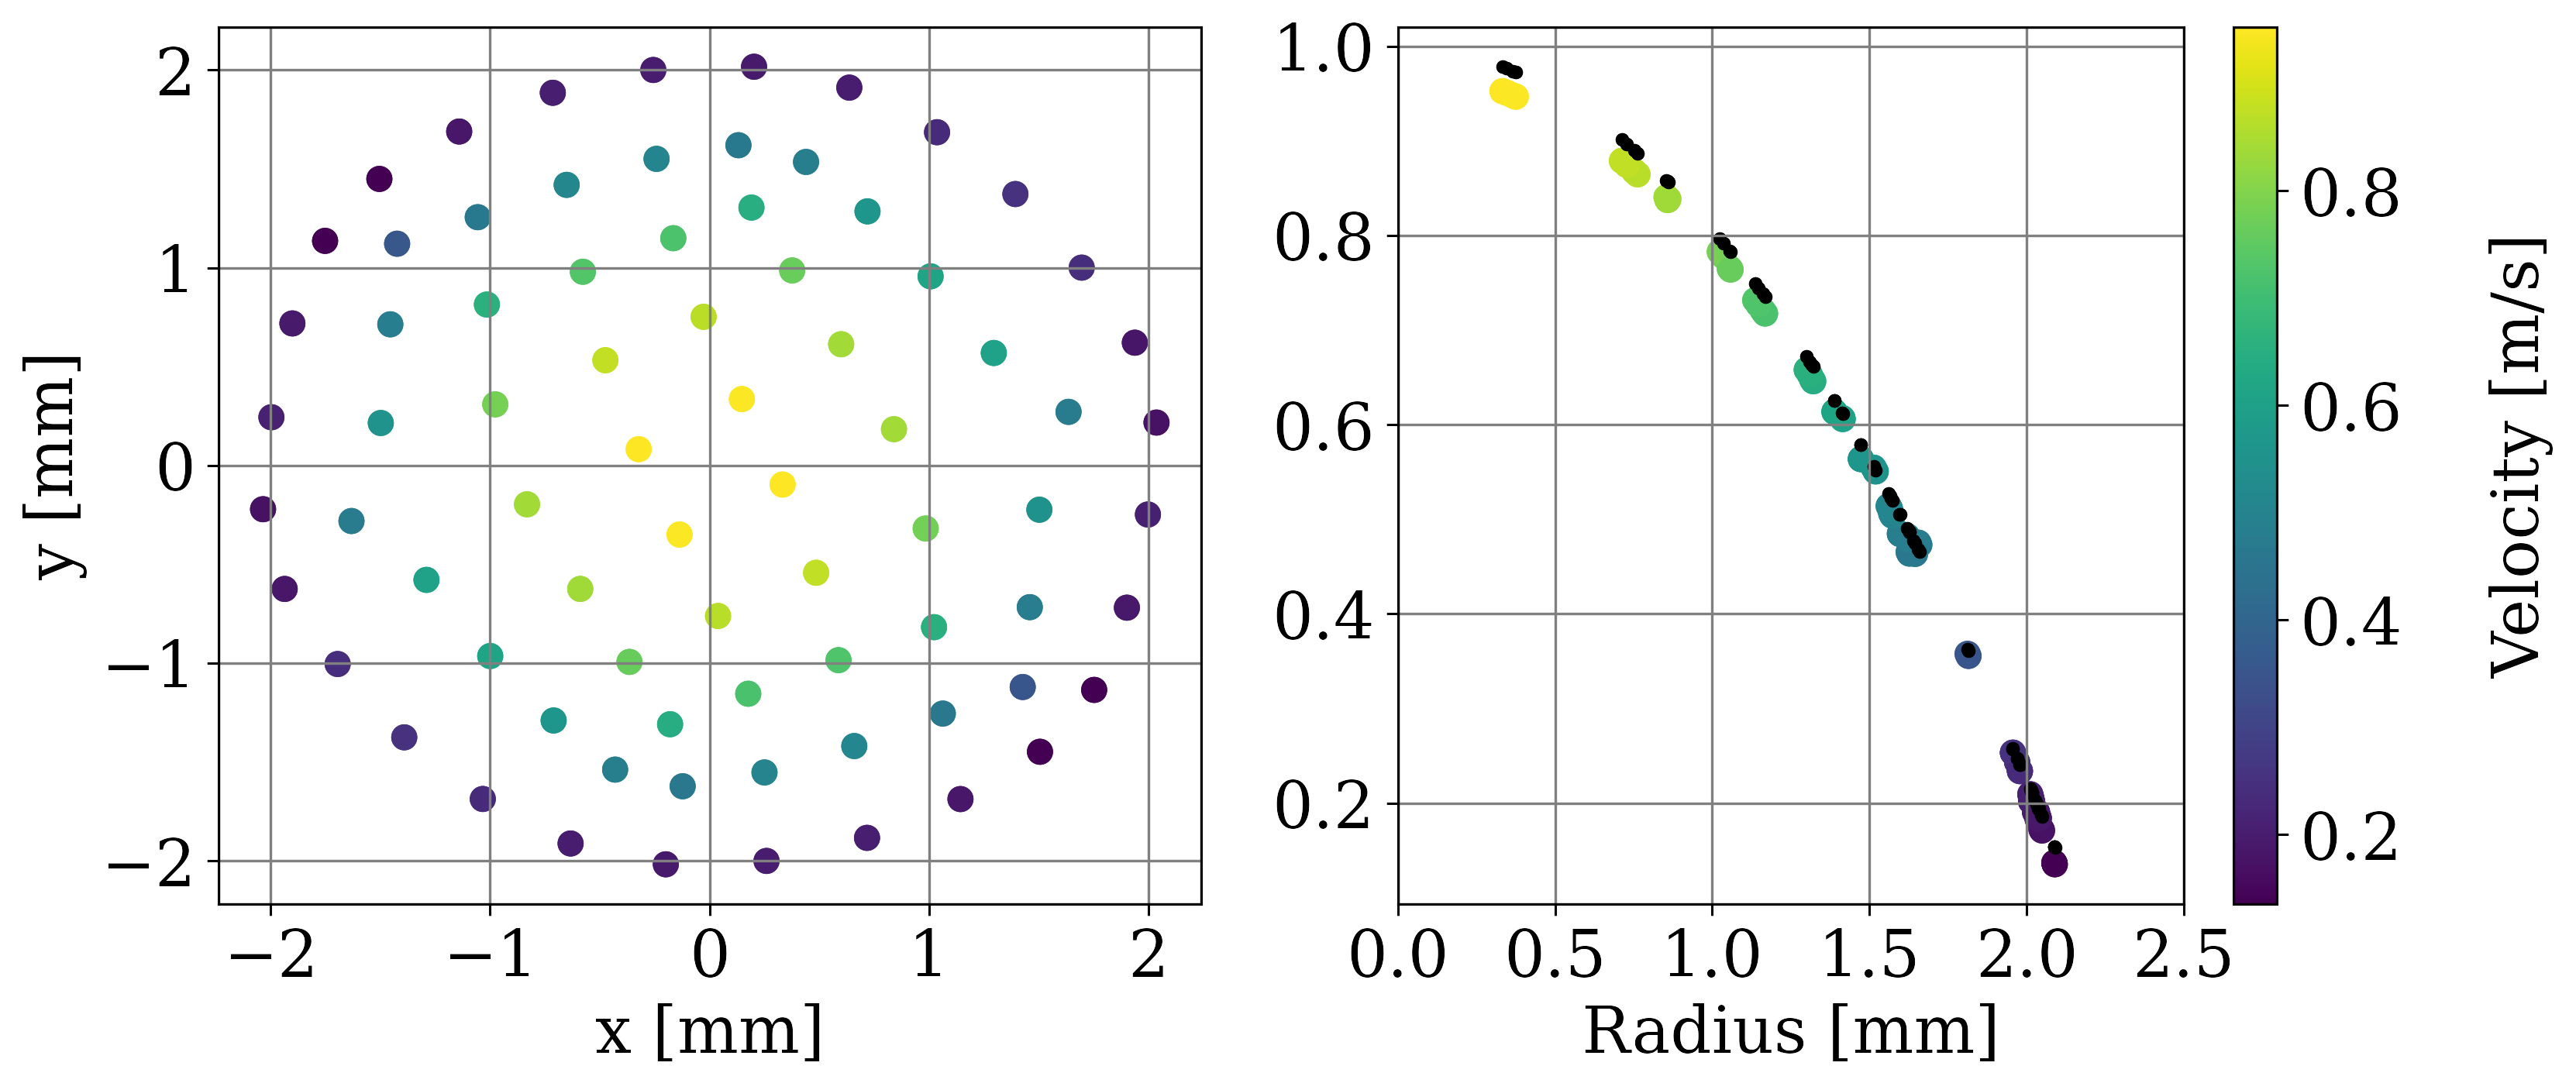
\includegraphics[width=\textwidth]{figures/code_verification/poiseuille/U_scatter_radial_z5mm_M0.png}
    \caption{Coarse Mesh}
    \label{fig:sub1}
  \end{subfigure}
  \hfill
  \begin{subfigure}[b]{0.5\textwidth}
    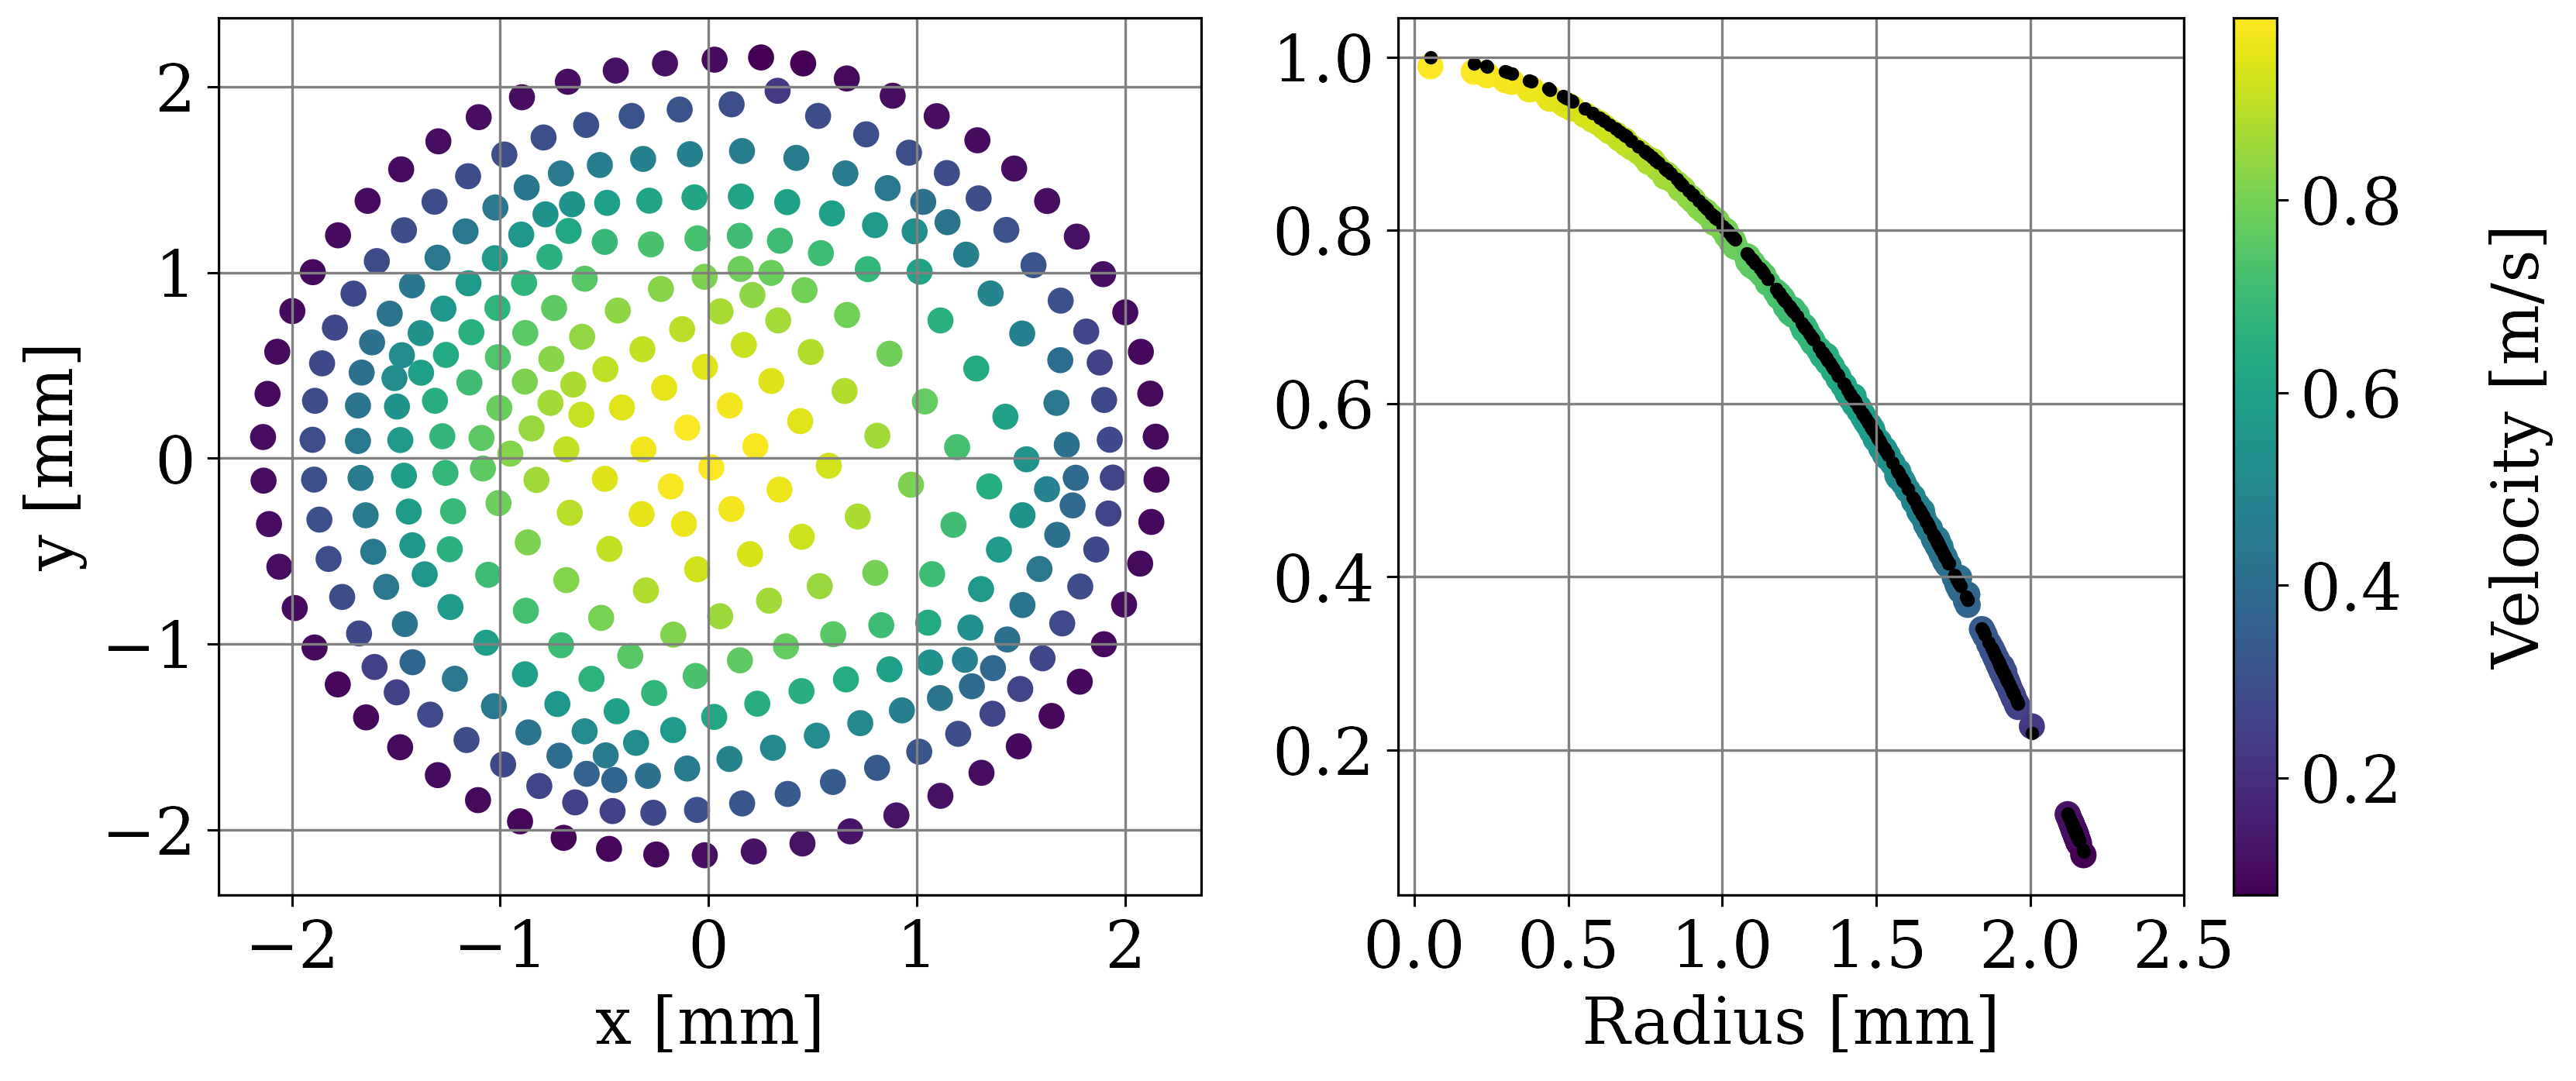
\includegraphics[width=\textwidth]{figures/code_verification/poiseuille/U_scatter_radial_z5mm_M1.png}
    \caption{Medium Mesh}
    \label{fig:sub2}
  \end{subfigure}
  \hfill
  \begin{subfigure}[b]{0.5\textwidth}
    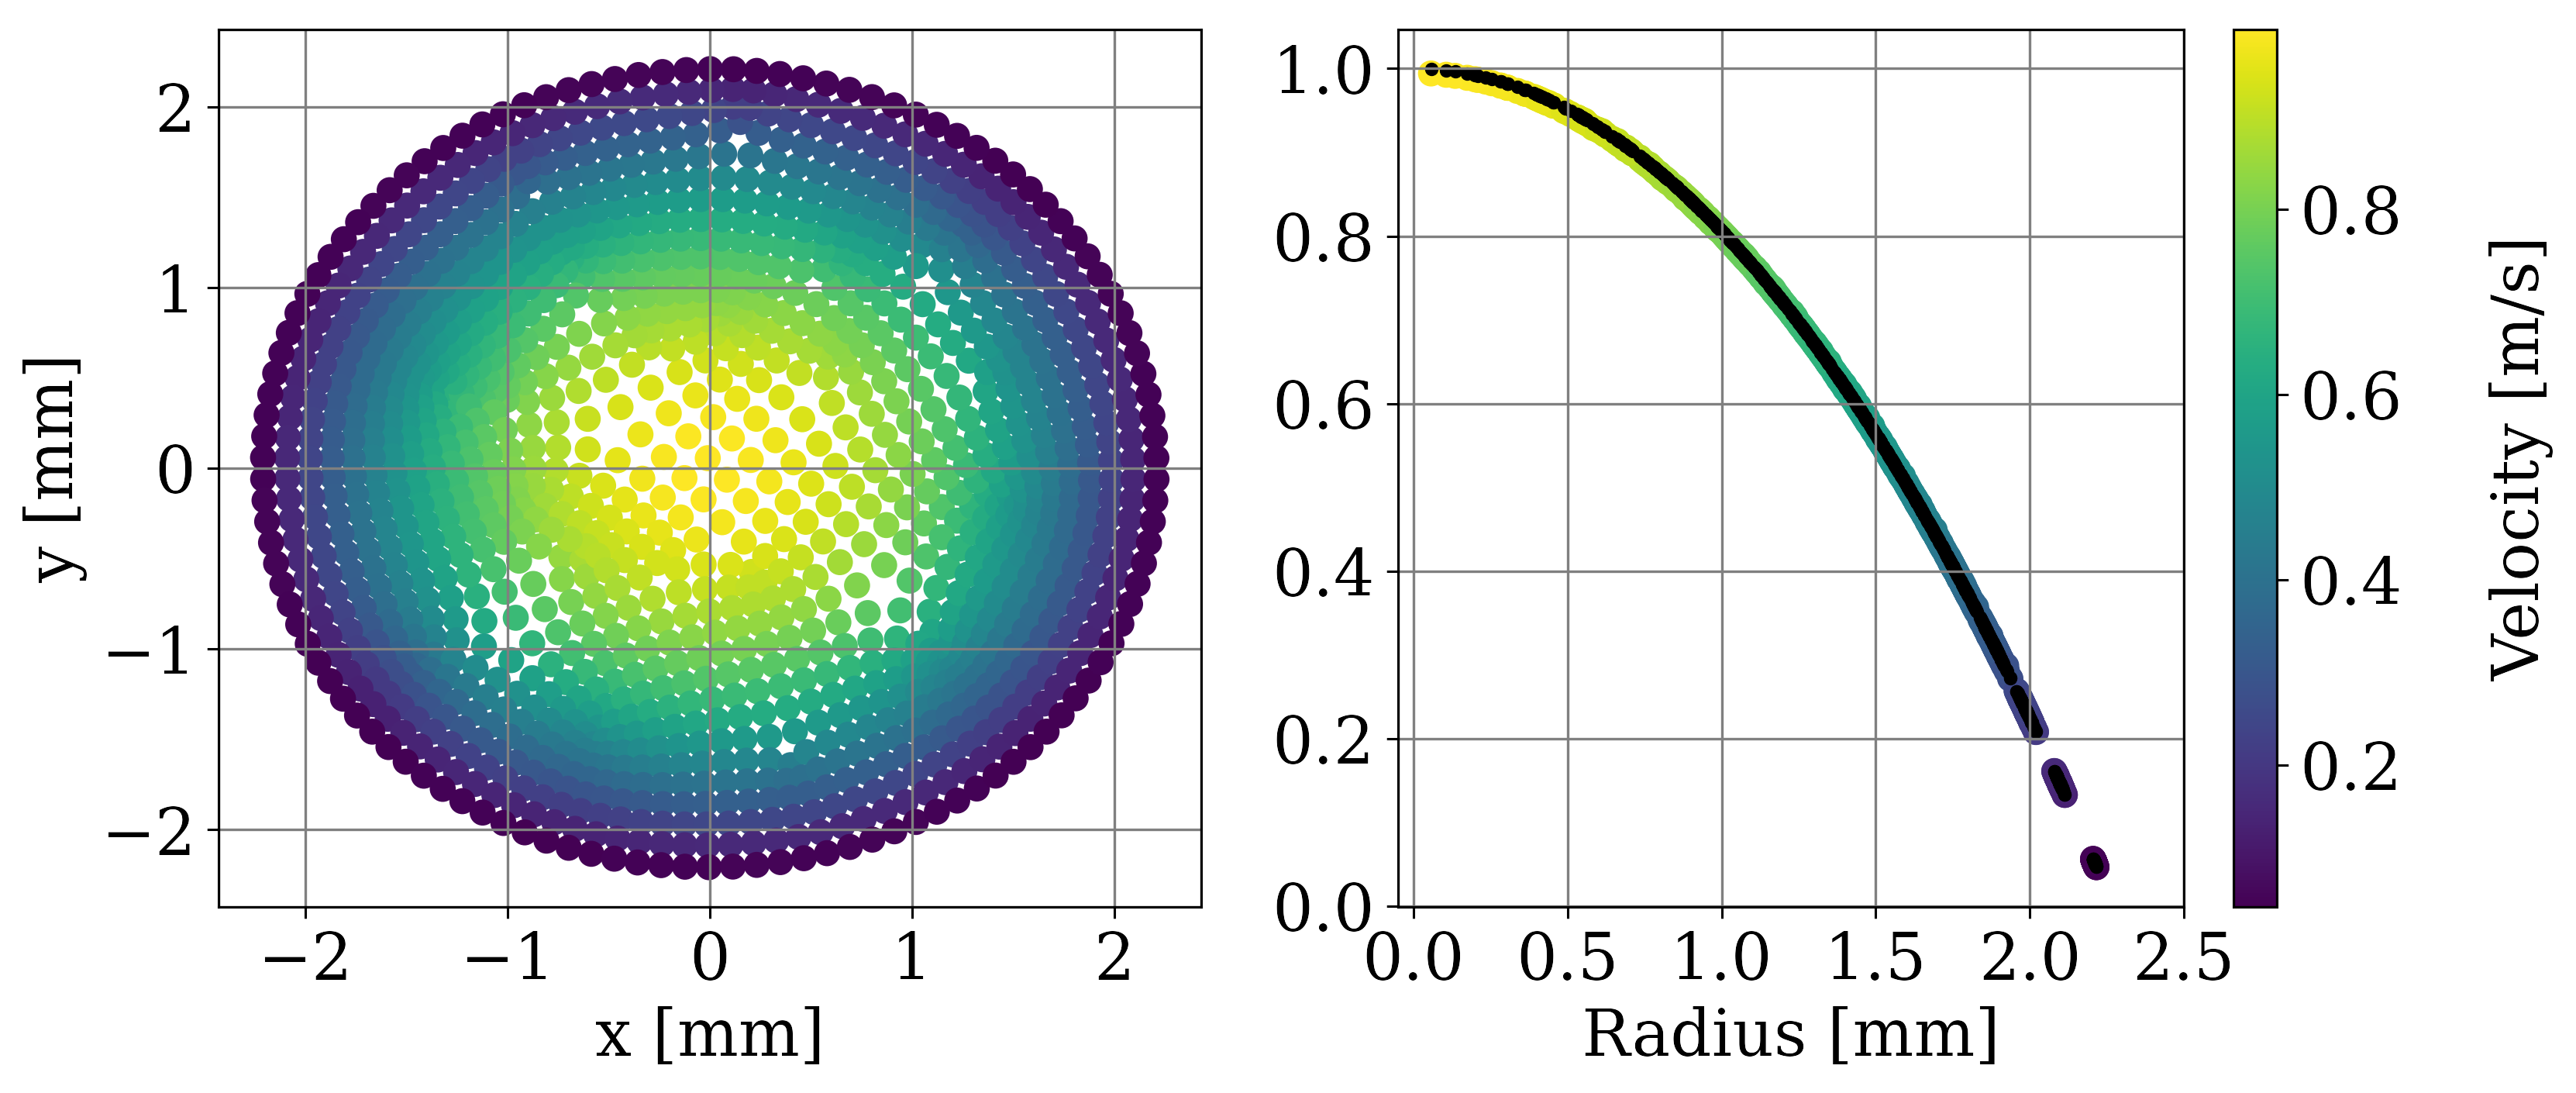
\includegraphics[width=\textwidth]{figures/code_verification/poiseuille/U_scatter_radial_z5mm_M2.png}
    \caption{Fine Mesh}
    \label{fig:sub3}
  \end{subfigure}
  \caption{Simulated hydrodynamic model axial velocity by radial position at $QoI_{\text{hydro}}$, overlaid with the analytical Hagen-Poiseuille solution (black points).}
  \label{fig:scatterVelocity}
\end{figure}

The normalized $L_2$ error was evaluated for each mesh and plotted against representative cell length (Figure~\ref{fig:errorVsLength}). The error decreases consistently with mesh refinement, yielding an observed order of convergence of $p = 1.95$. This behavior is consistent with the expected second-order accuracy of the spatial discretization scheme. These results confirm that the numerical solver accurately represents the analytical velocity field.

\begin{figure}[htbp!]
    \centering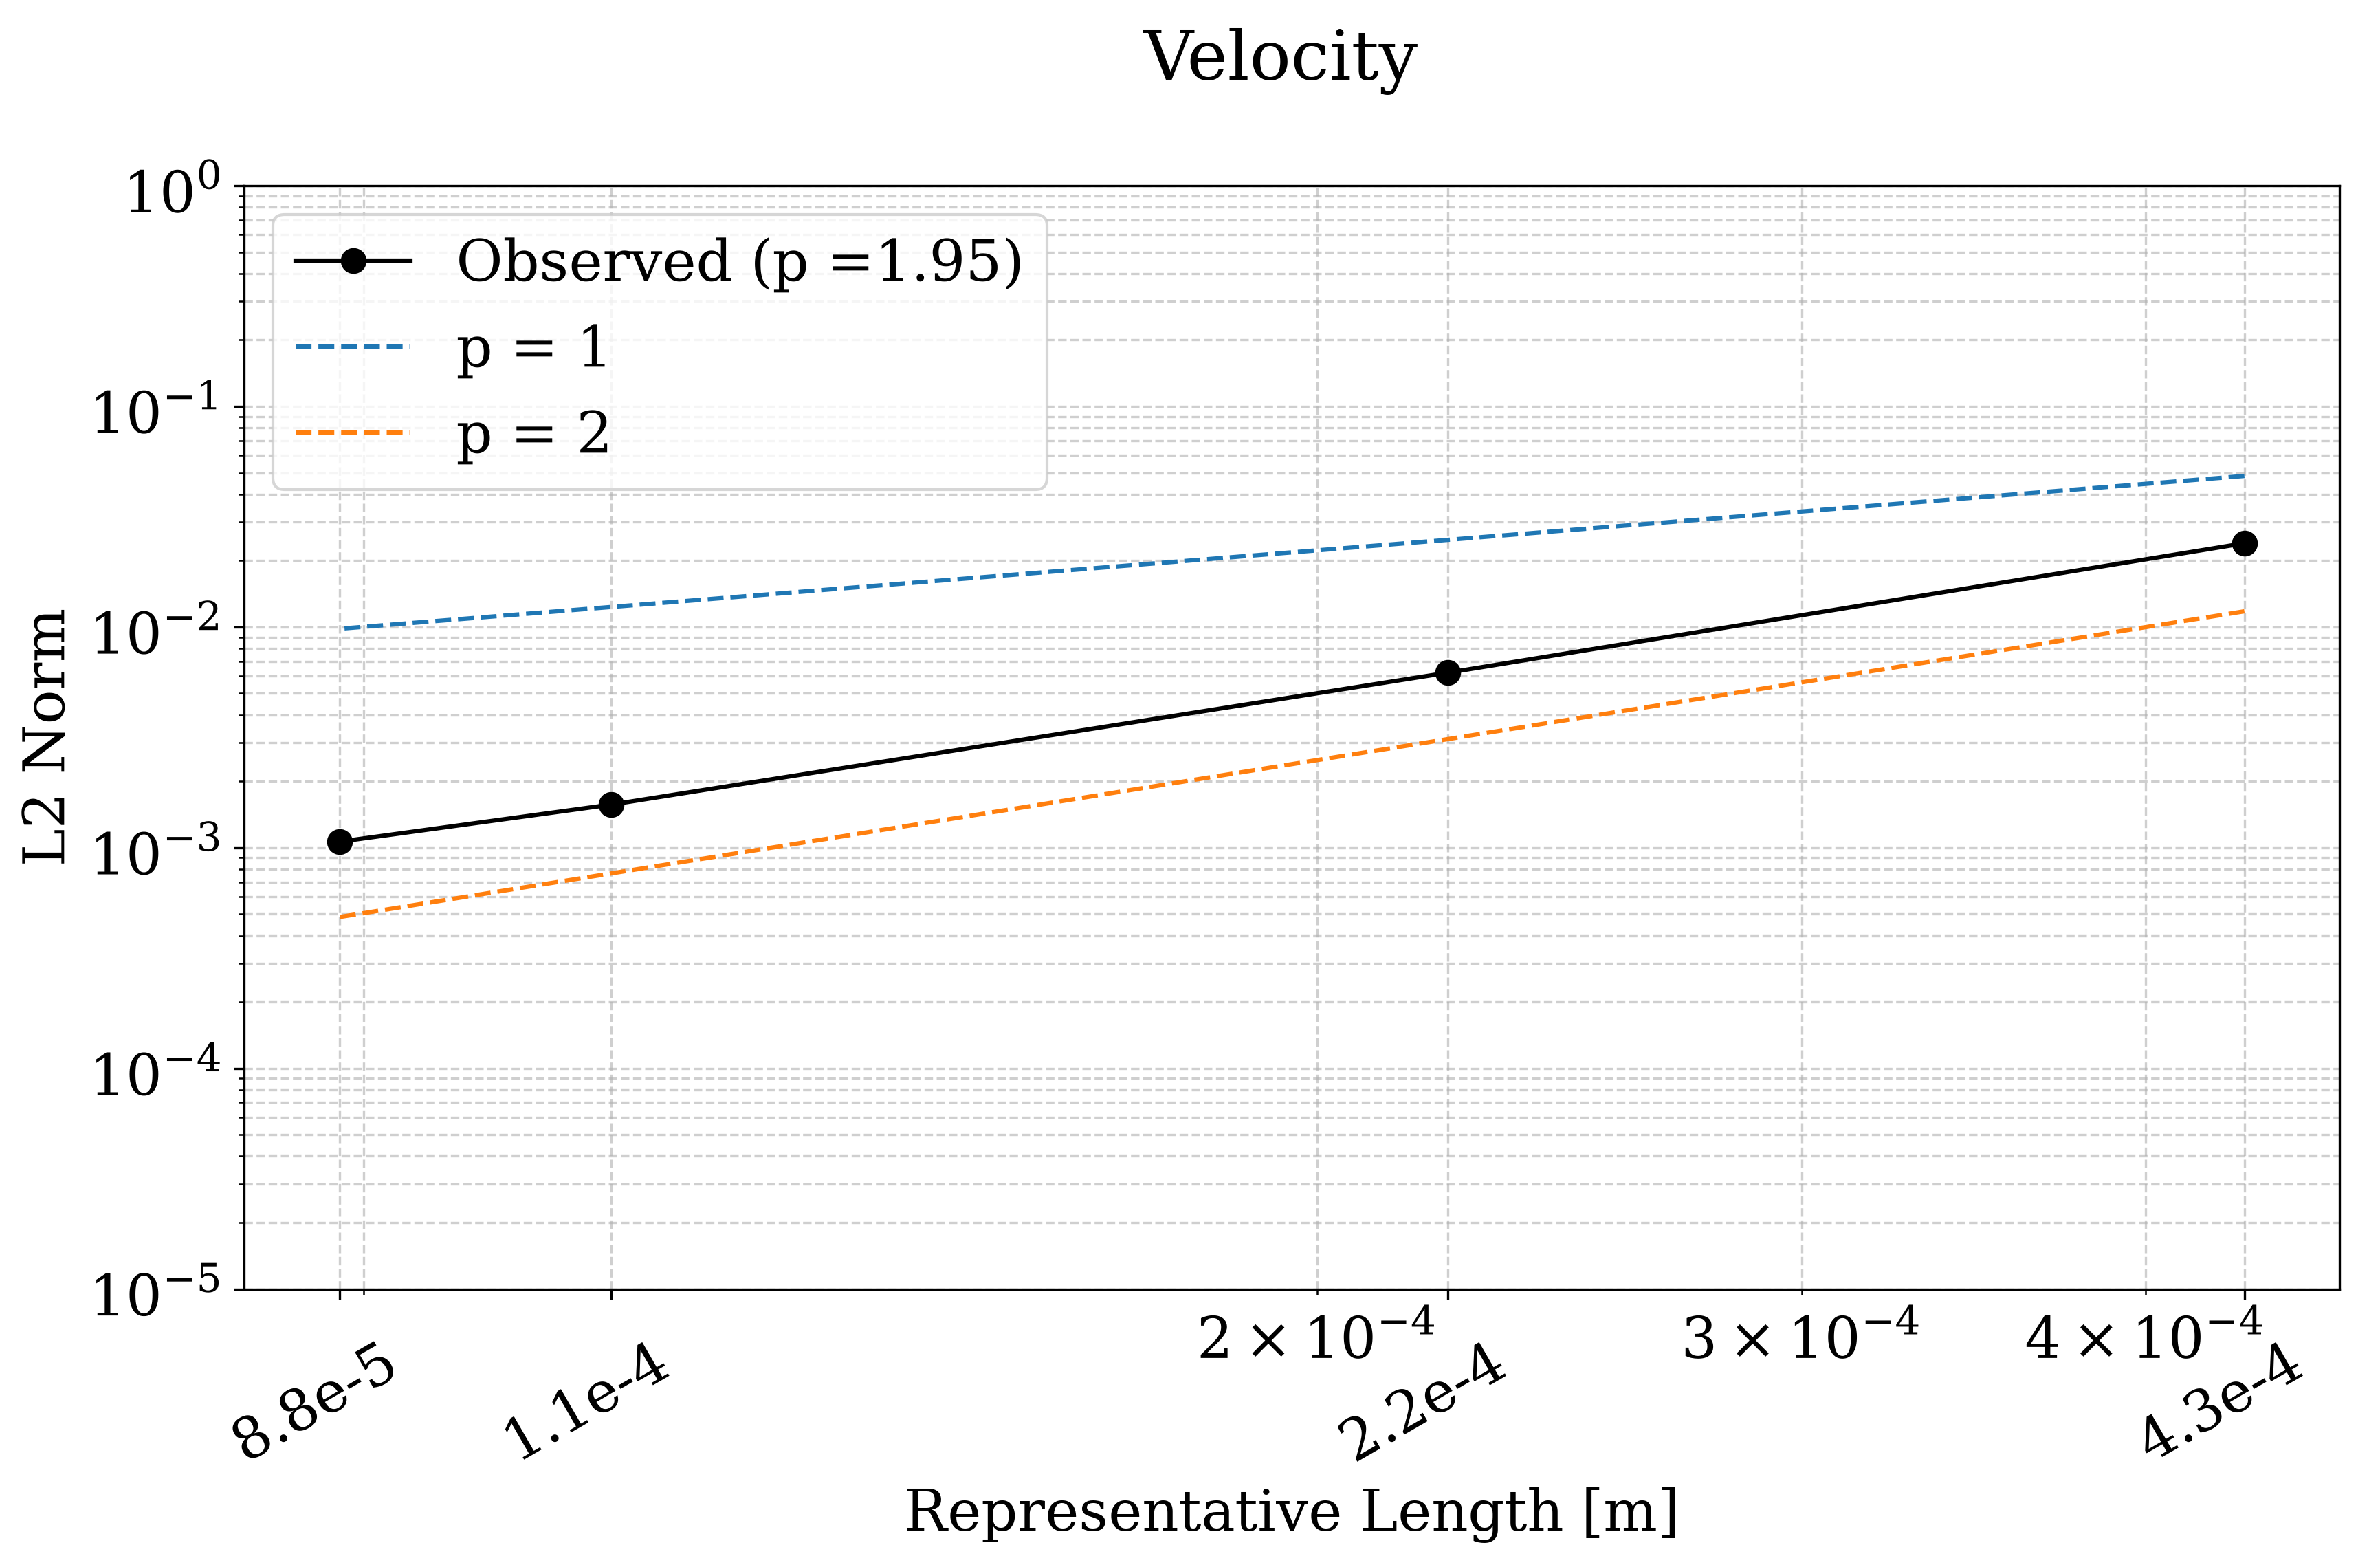
\includegraphics[width=0.95 \linewidth]{figures/code_verification/poiseuille/U_L2Norm_Observed_p.png} 
        \caption{Hydrodynamic model velocity $L_2$ error by representative cell length.}
        \label{fig:errorVsLength}
\end{figure}

\subsubsection{Radial Conduction Model}
To verify the implementation of the solid energy equation, a steady-state conduction-dominated configuration was constructed with the \texttt{chtMultiRegionFoam} solver. The problem was formulated such that the governing equations reduce to a one-dimensional radial conduction with uniform volumetric heat generation in the solid, enabling direct comparison with the analytical solution. Spatial convergence was assessed using three progressively refined meshes with representative cell sizes of 0.14~mm, 0.071~mm, and 0.035~mm. Temperature was evaluated at a cross-sectional plane sufficiently far from inlet and outlet effects to ensure a fully developed radial profile, presented in Figure~\ref{fig:scatterTemperature}.

% #Extra info: 
% Three refined meshes were used a coarse mesh with 18,000 nodes and a representative cell length of 0.14mm, a medium mesh with 144,000 nodes and a representative length of 0.071 mm, and a fine mesh with 1,152,000 nodes and a representative length of 0.035 mm. Axial Temperature are sampled across $z$ = 67.5 mm, a location far enough from the inlet and outlet. 

\begin{figure}[htbp]
  \centering
  \begin{subfigure}[b]{0.5\textwidth}
    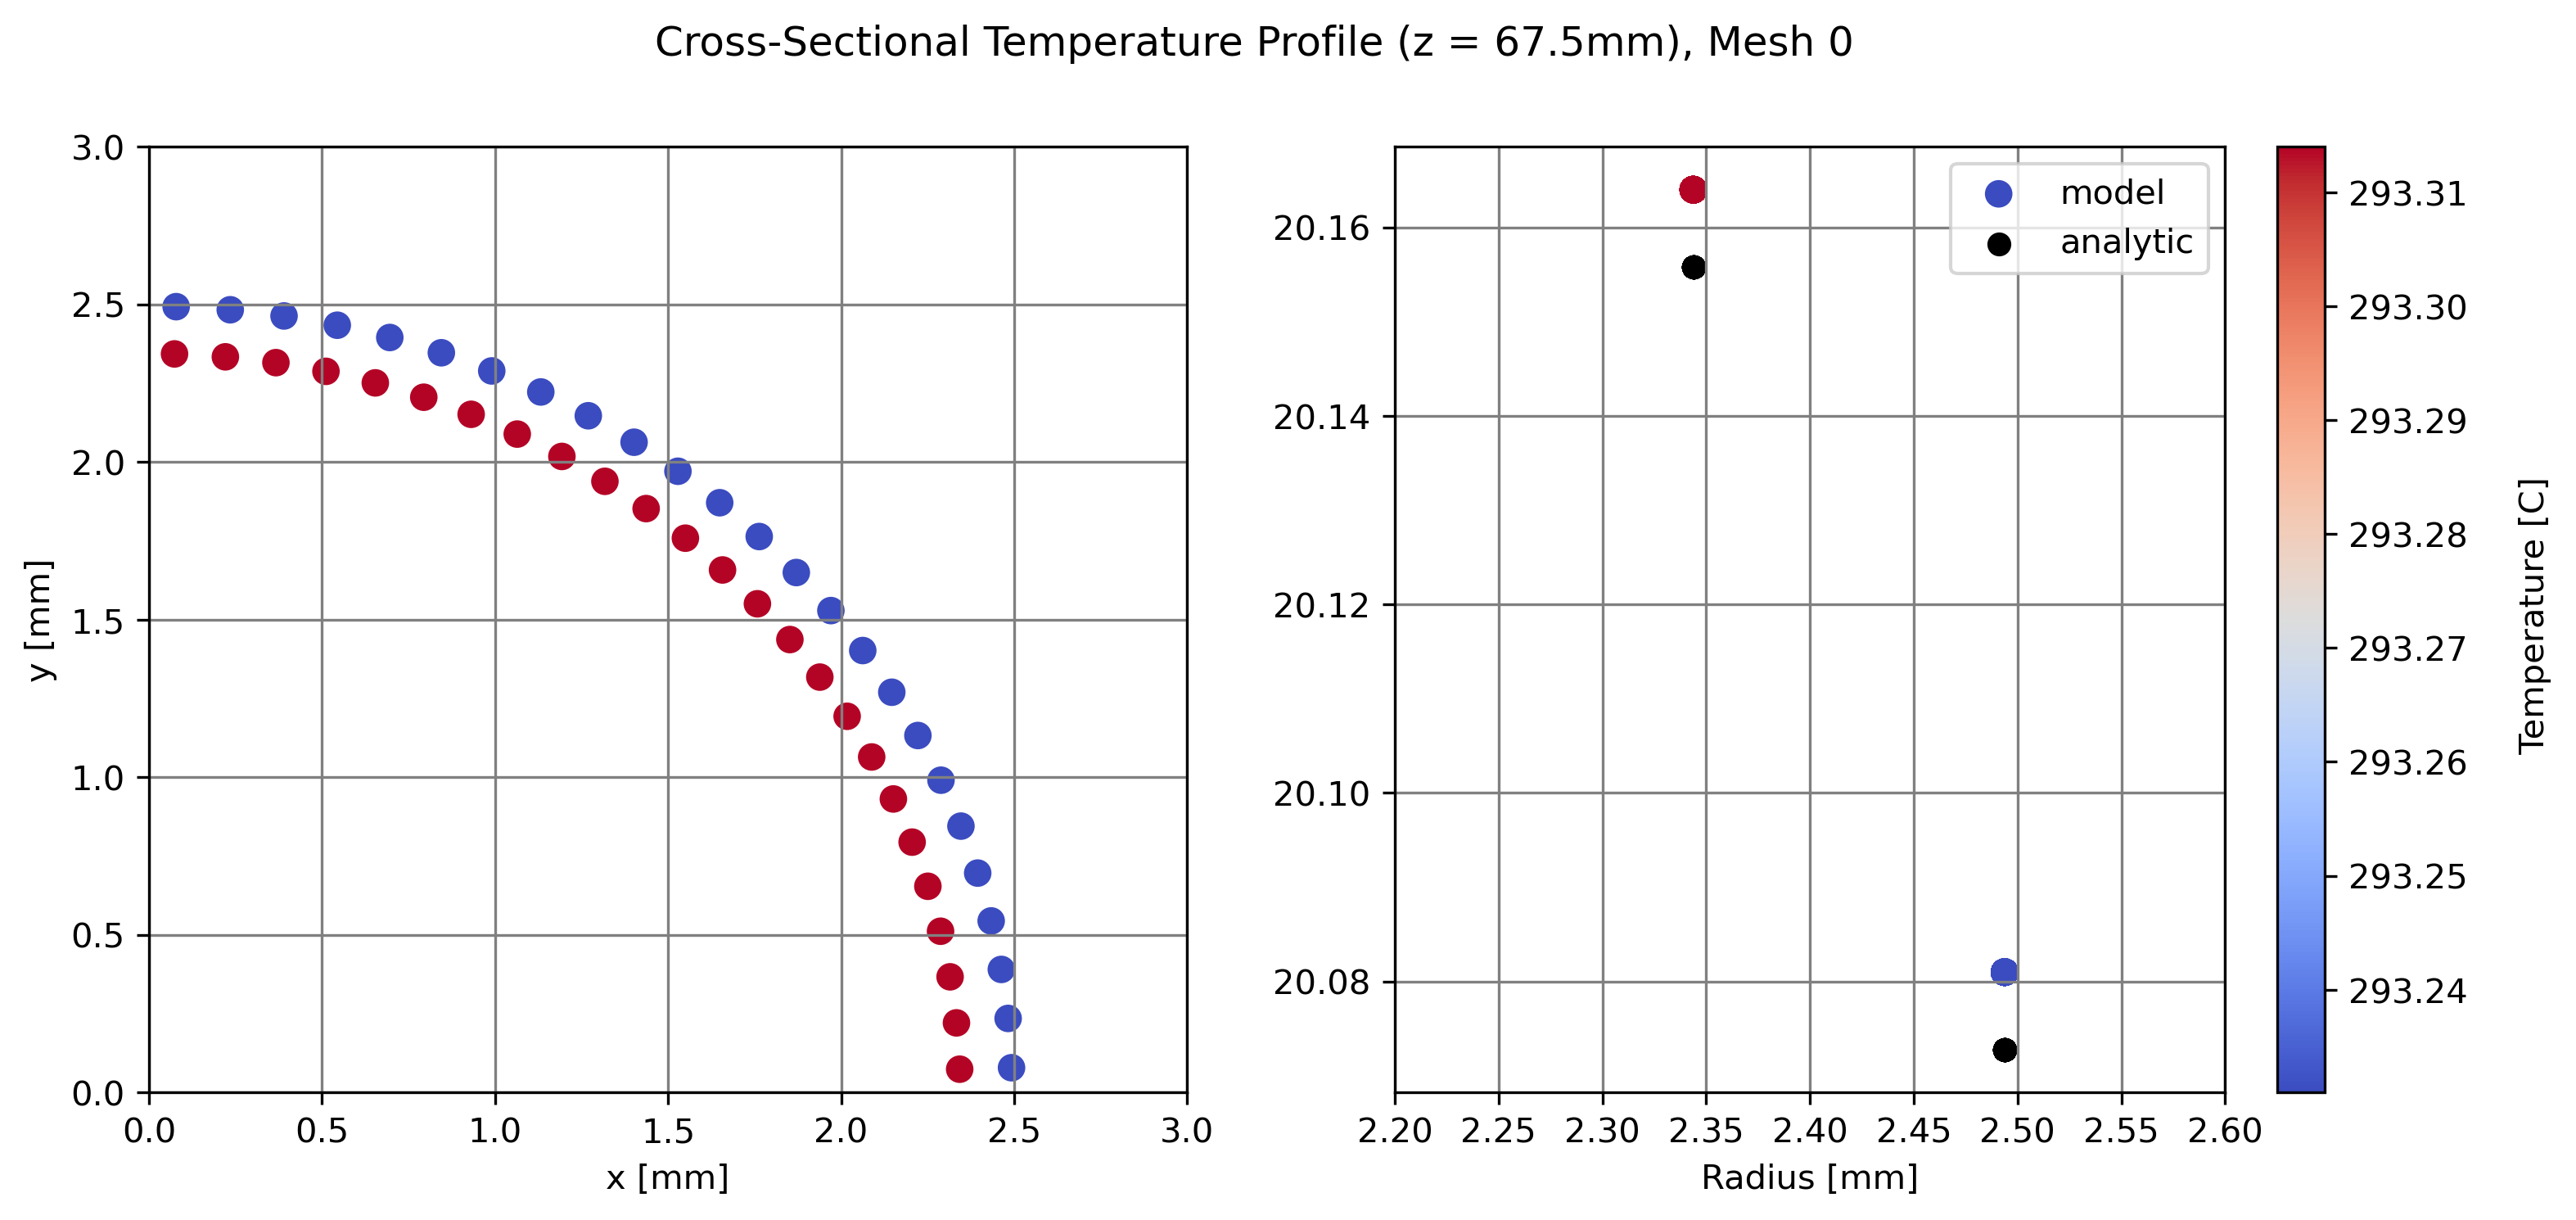
\includegraphics[width=\textwidth]{figures/heatsource/T_scatter_radial_z67.5mm_M0.png}
    \caption{Coarse mesh. }
    \label{fig:sub1T}
  \end{subfigure}
  \hfill
  \begin{subfigure}[b]{0.5\textwidth}
    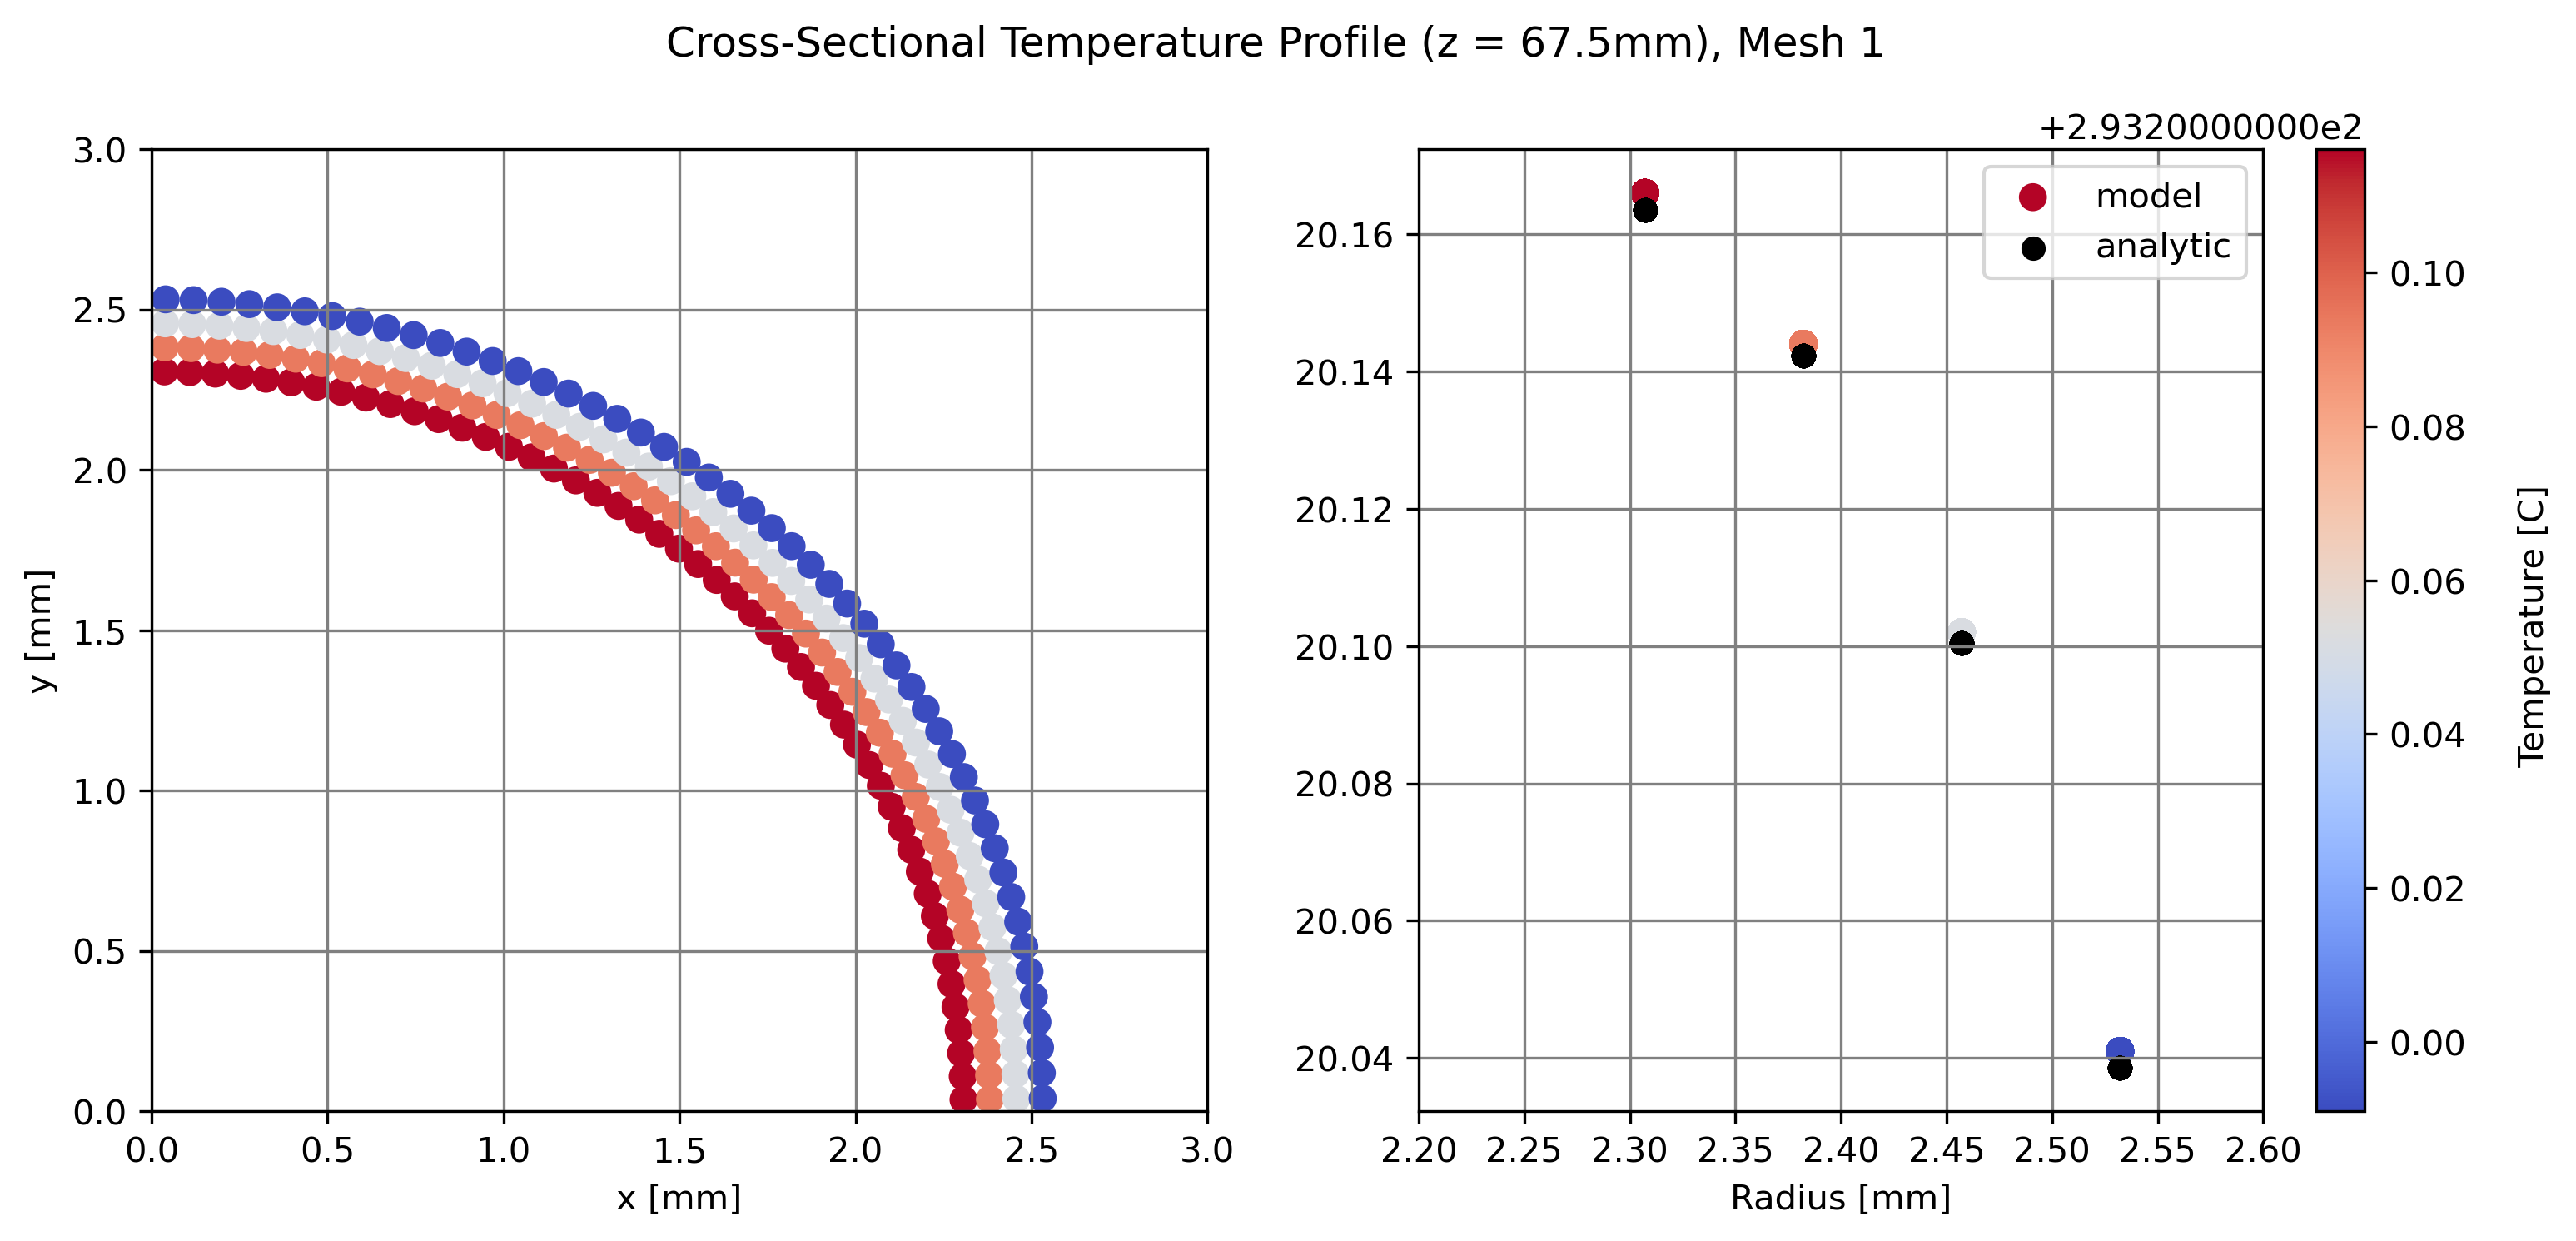
\includegraphics[width=\textwidth]{figures/heatsource/T_scatter_radial_z67.5mm_M1.png}
    \caption{Medium mesh.}
    \label{fig:sub2T}
  \end{subfigure}
  \hfill
  \begin{subfigure}[b]{0.5\textwidth}
    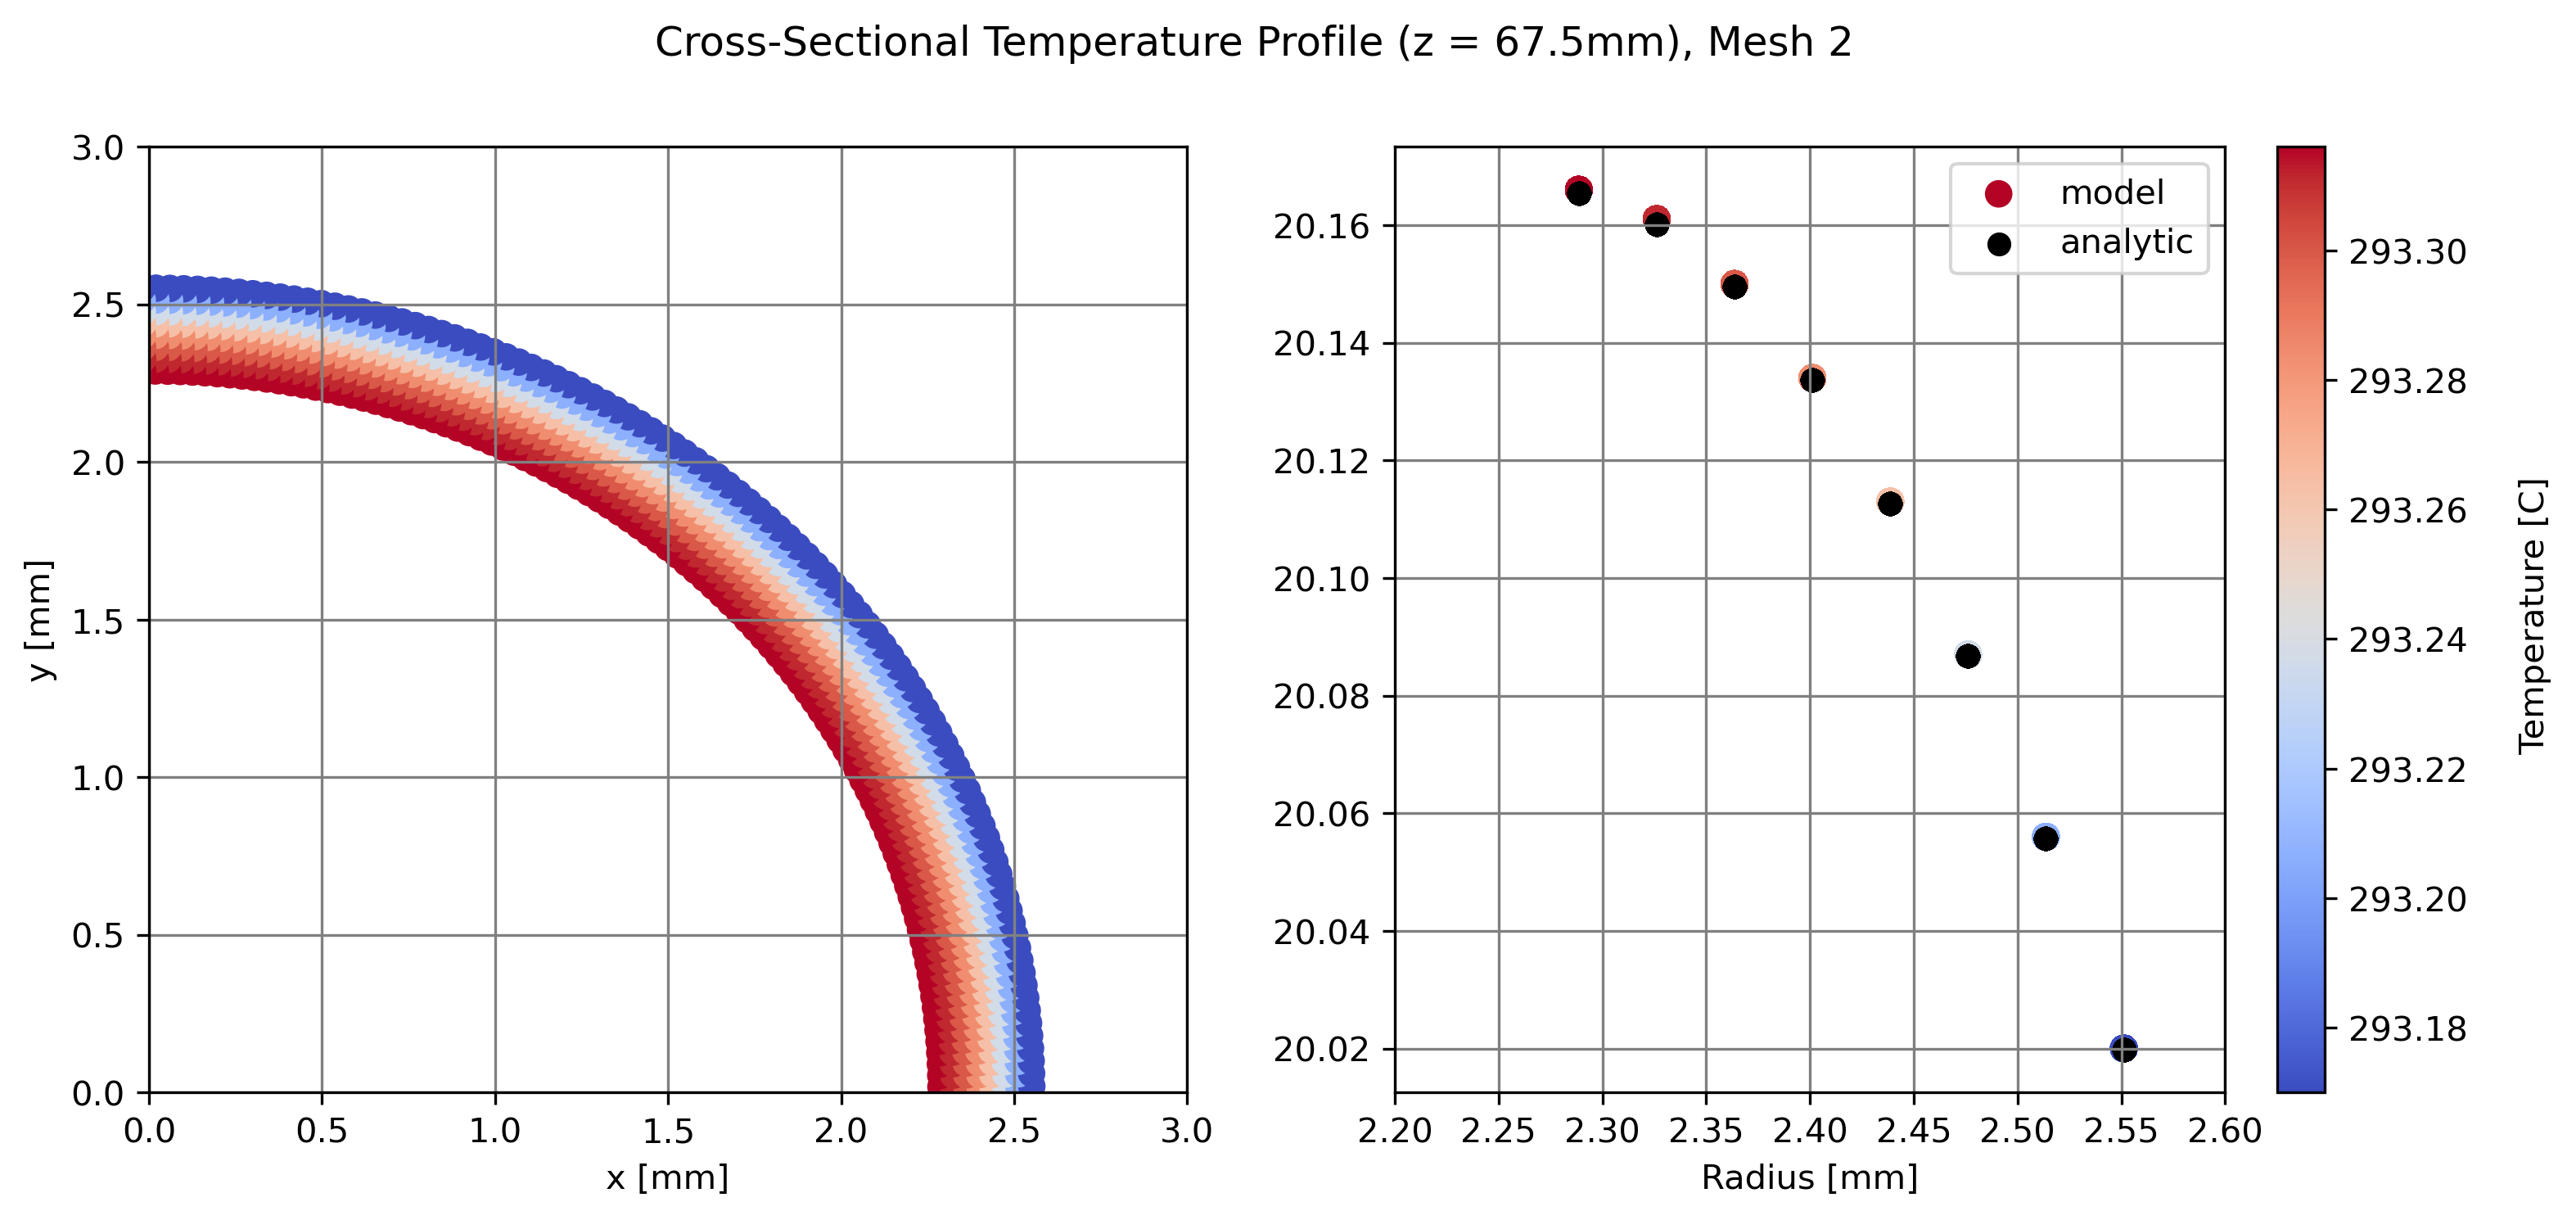
\includegraphics[width=\textwidth]{figures/heatsource/T_scatter_radial_z67.5mm_M2.png}
    \caption{Fine mesh.}
    \label{fig:sub3T}
  \end{subfigure}
  \caption{Radial conduction model simulated temperature by radial position at $QoI_{\text{cond}}$, overlaid with the analytical solution (black points).}
  \label{fig:scatterTemperature}
\end{figure}

Figure~\ref{fig:scatterTemperature} shows that the numerical temperature field converges toward the analytical solution as mesh resolution increases. The coarse mesh exhibits noticeable deviation from the analytical profile, while refinement reduces this discrepancy and the fine mesh achieves near pointwise agreement across the radius. The normalized $L_2$ error was evaluated for each mesh and plotted against representative cell length (Figure~\ref{fig:l2normTempInterface}). The error decreases consistently with mesh refinement, producing an observed order of convergence of $p = 2.08$, which is consistent with the expected second-order spatial accuracy of the discretization scheme. The error magnitude decreases from $\mathcal{O}(10^{-4})$ to $\mathcal{O}(10^{-6})$, indicating strong agreement with the analytical solution. These results confirm that the numerical implementation of the solid energy equation is correct and exhibits the expected convergence behavior under mesh refinement.

\begin{figure}[htbp!]
    \centering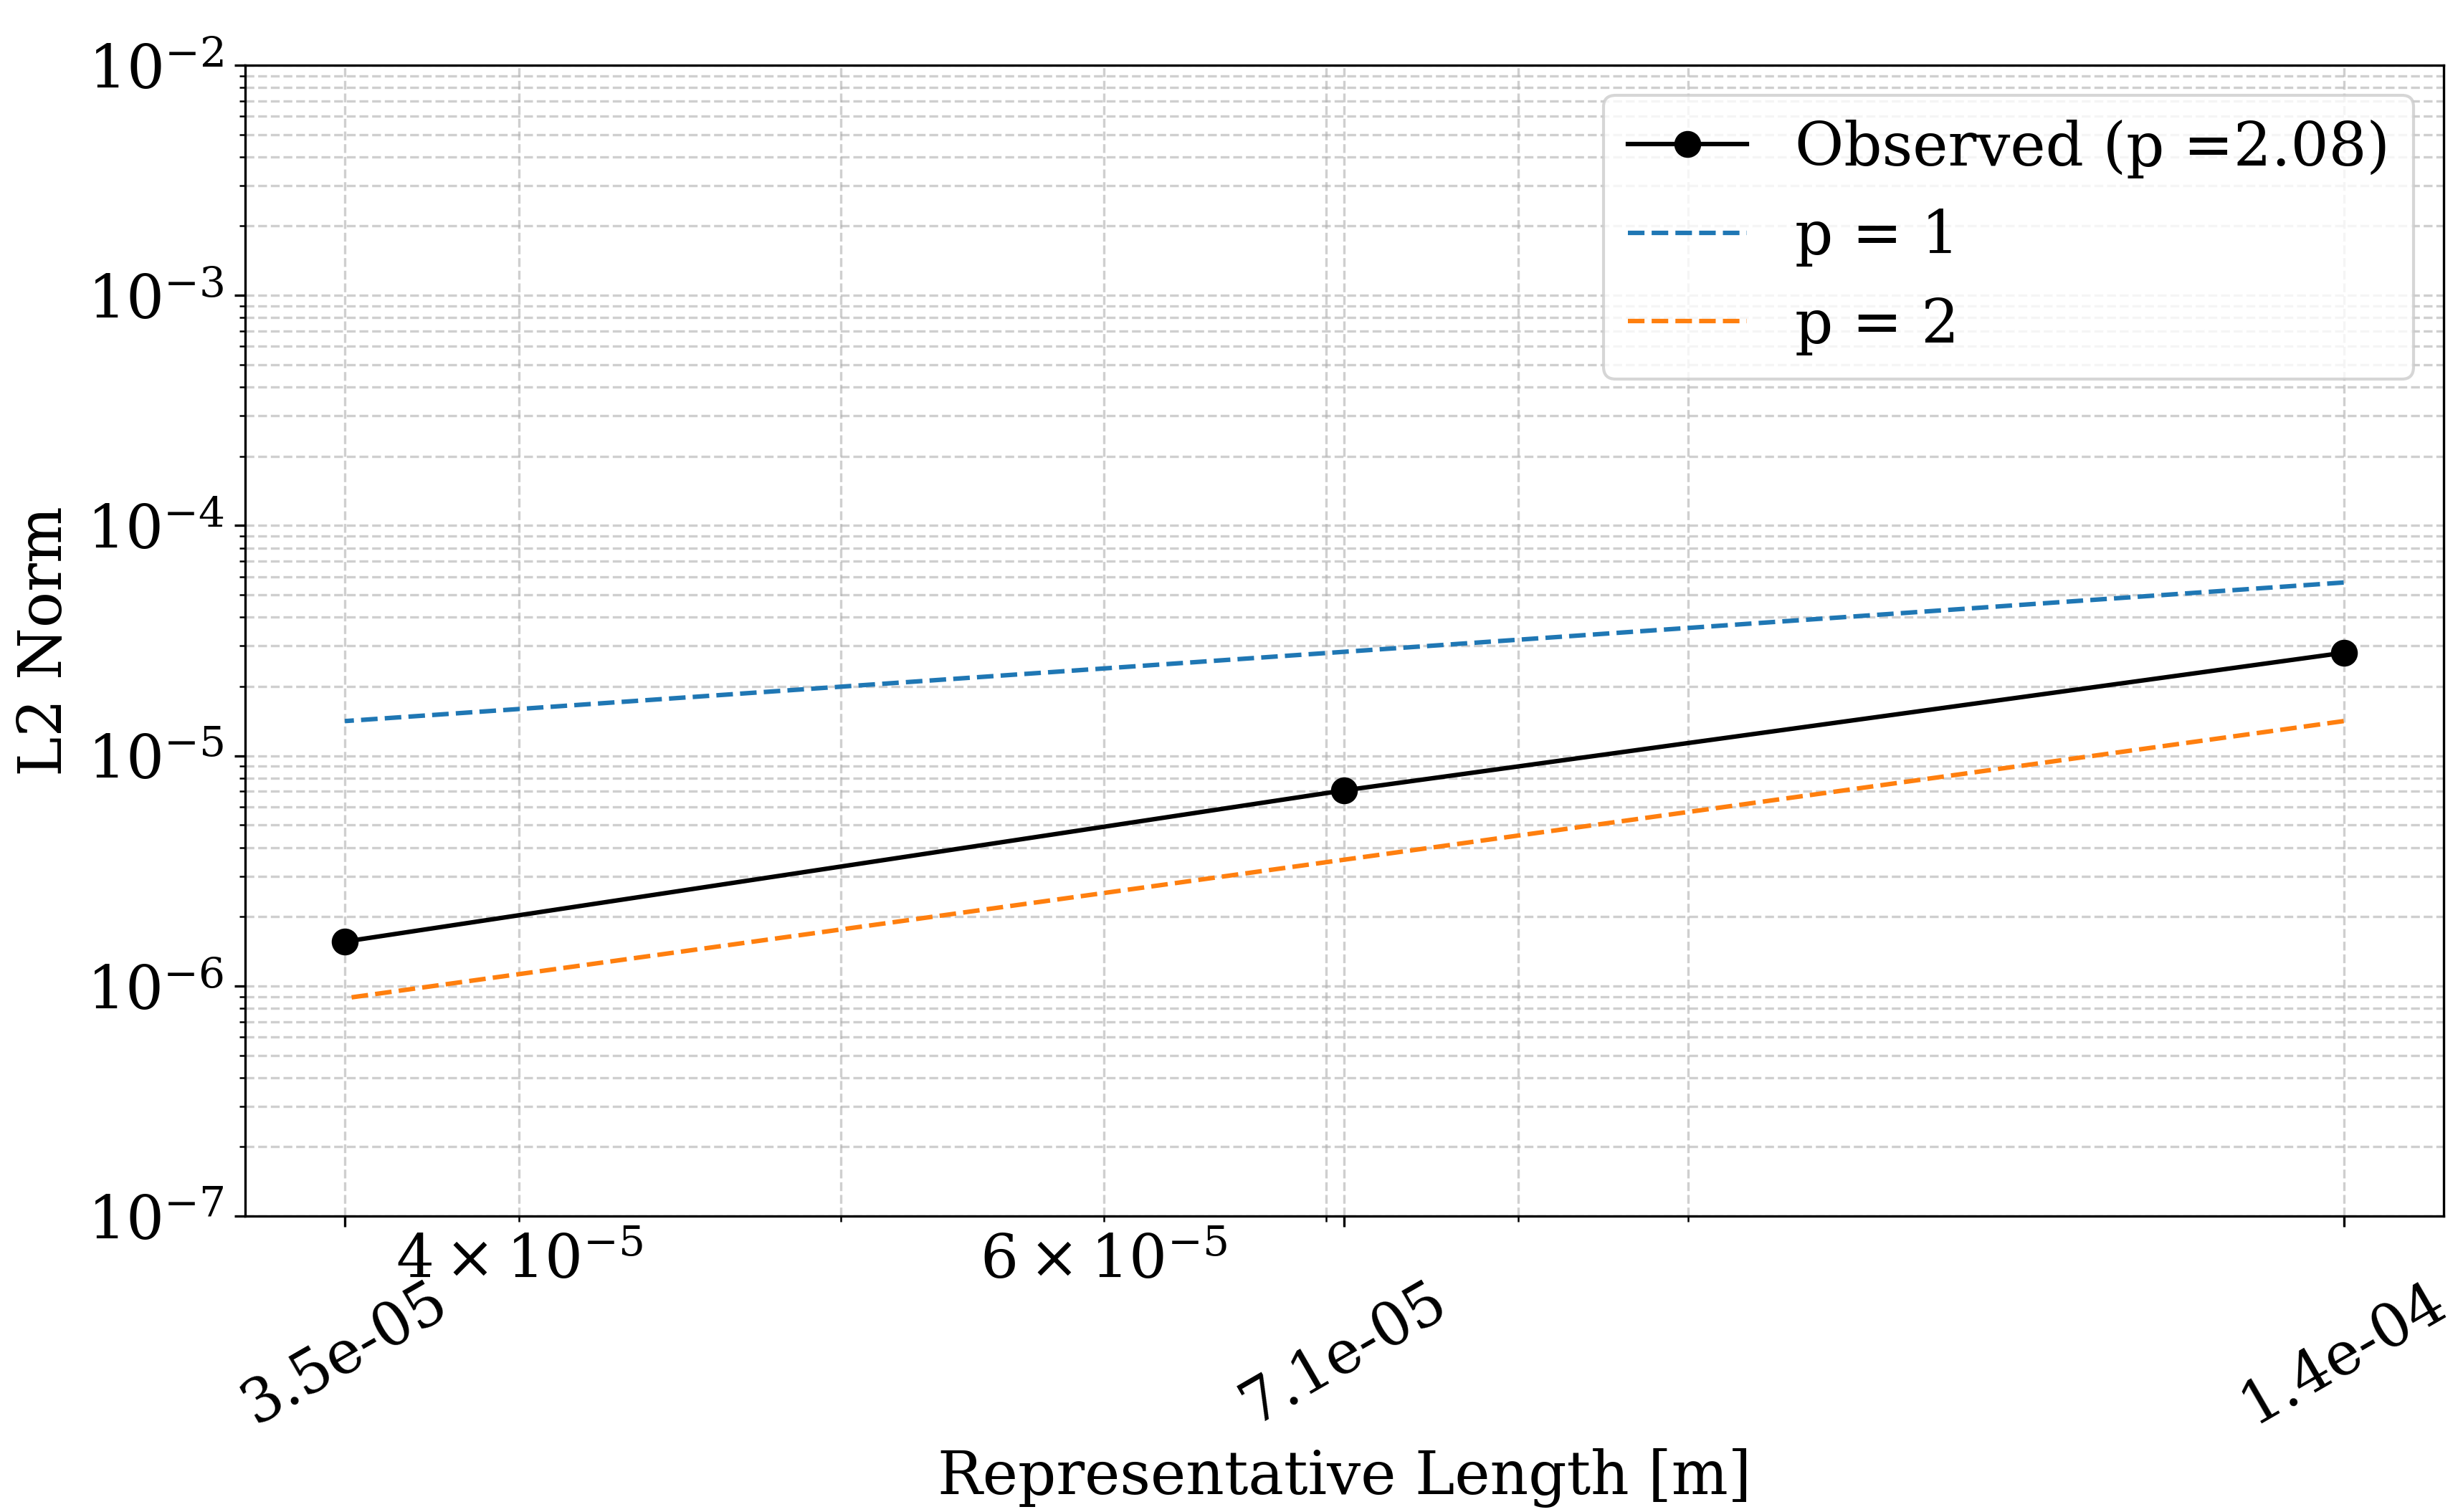
\includegraphics[width=0.95 \linewidth]{figures/heatsource/T_L2Norm_Observed_p.png} 
        \caption{Radial conduction model temperature $L_2$ error by representative cell length.}
        \label{fig:l2normTempInterface}
\end{figure}


\subsubsection{Transient Thermal Diffusion Verification}
Following isolated verification of the hydrodynamic and steady-state radial conduction models, a transient thermal diffusion case is used to bridge the isolated verification studies and the fully coupled transient conjugate heat transfer model. In order to reduce the governing energy equation to a radial diffusion problem the fluid velocity was set to zero. This isolates transient thermal transport and interface temperature transfer from the solid to the fluid region. The $L_2$ error is computed at a cross section, halfway along the heated fluid region, by comparing the simulated temperature, at each radial position, to the corresponding analytical radial temperature obtained from Eq.~\ref{eq:bessel_theta_solution} and Eq.~\ref{eq:dimensional_temperature}. Figure~\ref{fig:transientDiffusionConvergence} shows the normalized $L_2$ error as a function of representative cell size for multiple transient times. 

\begin{figure}[htbp!]
    \centering
    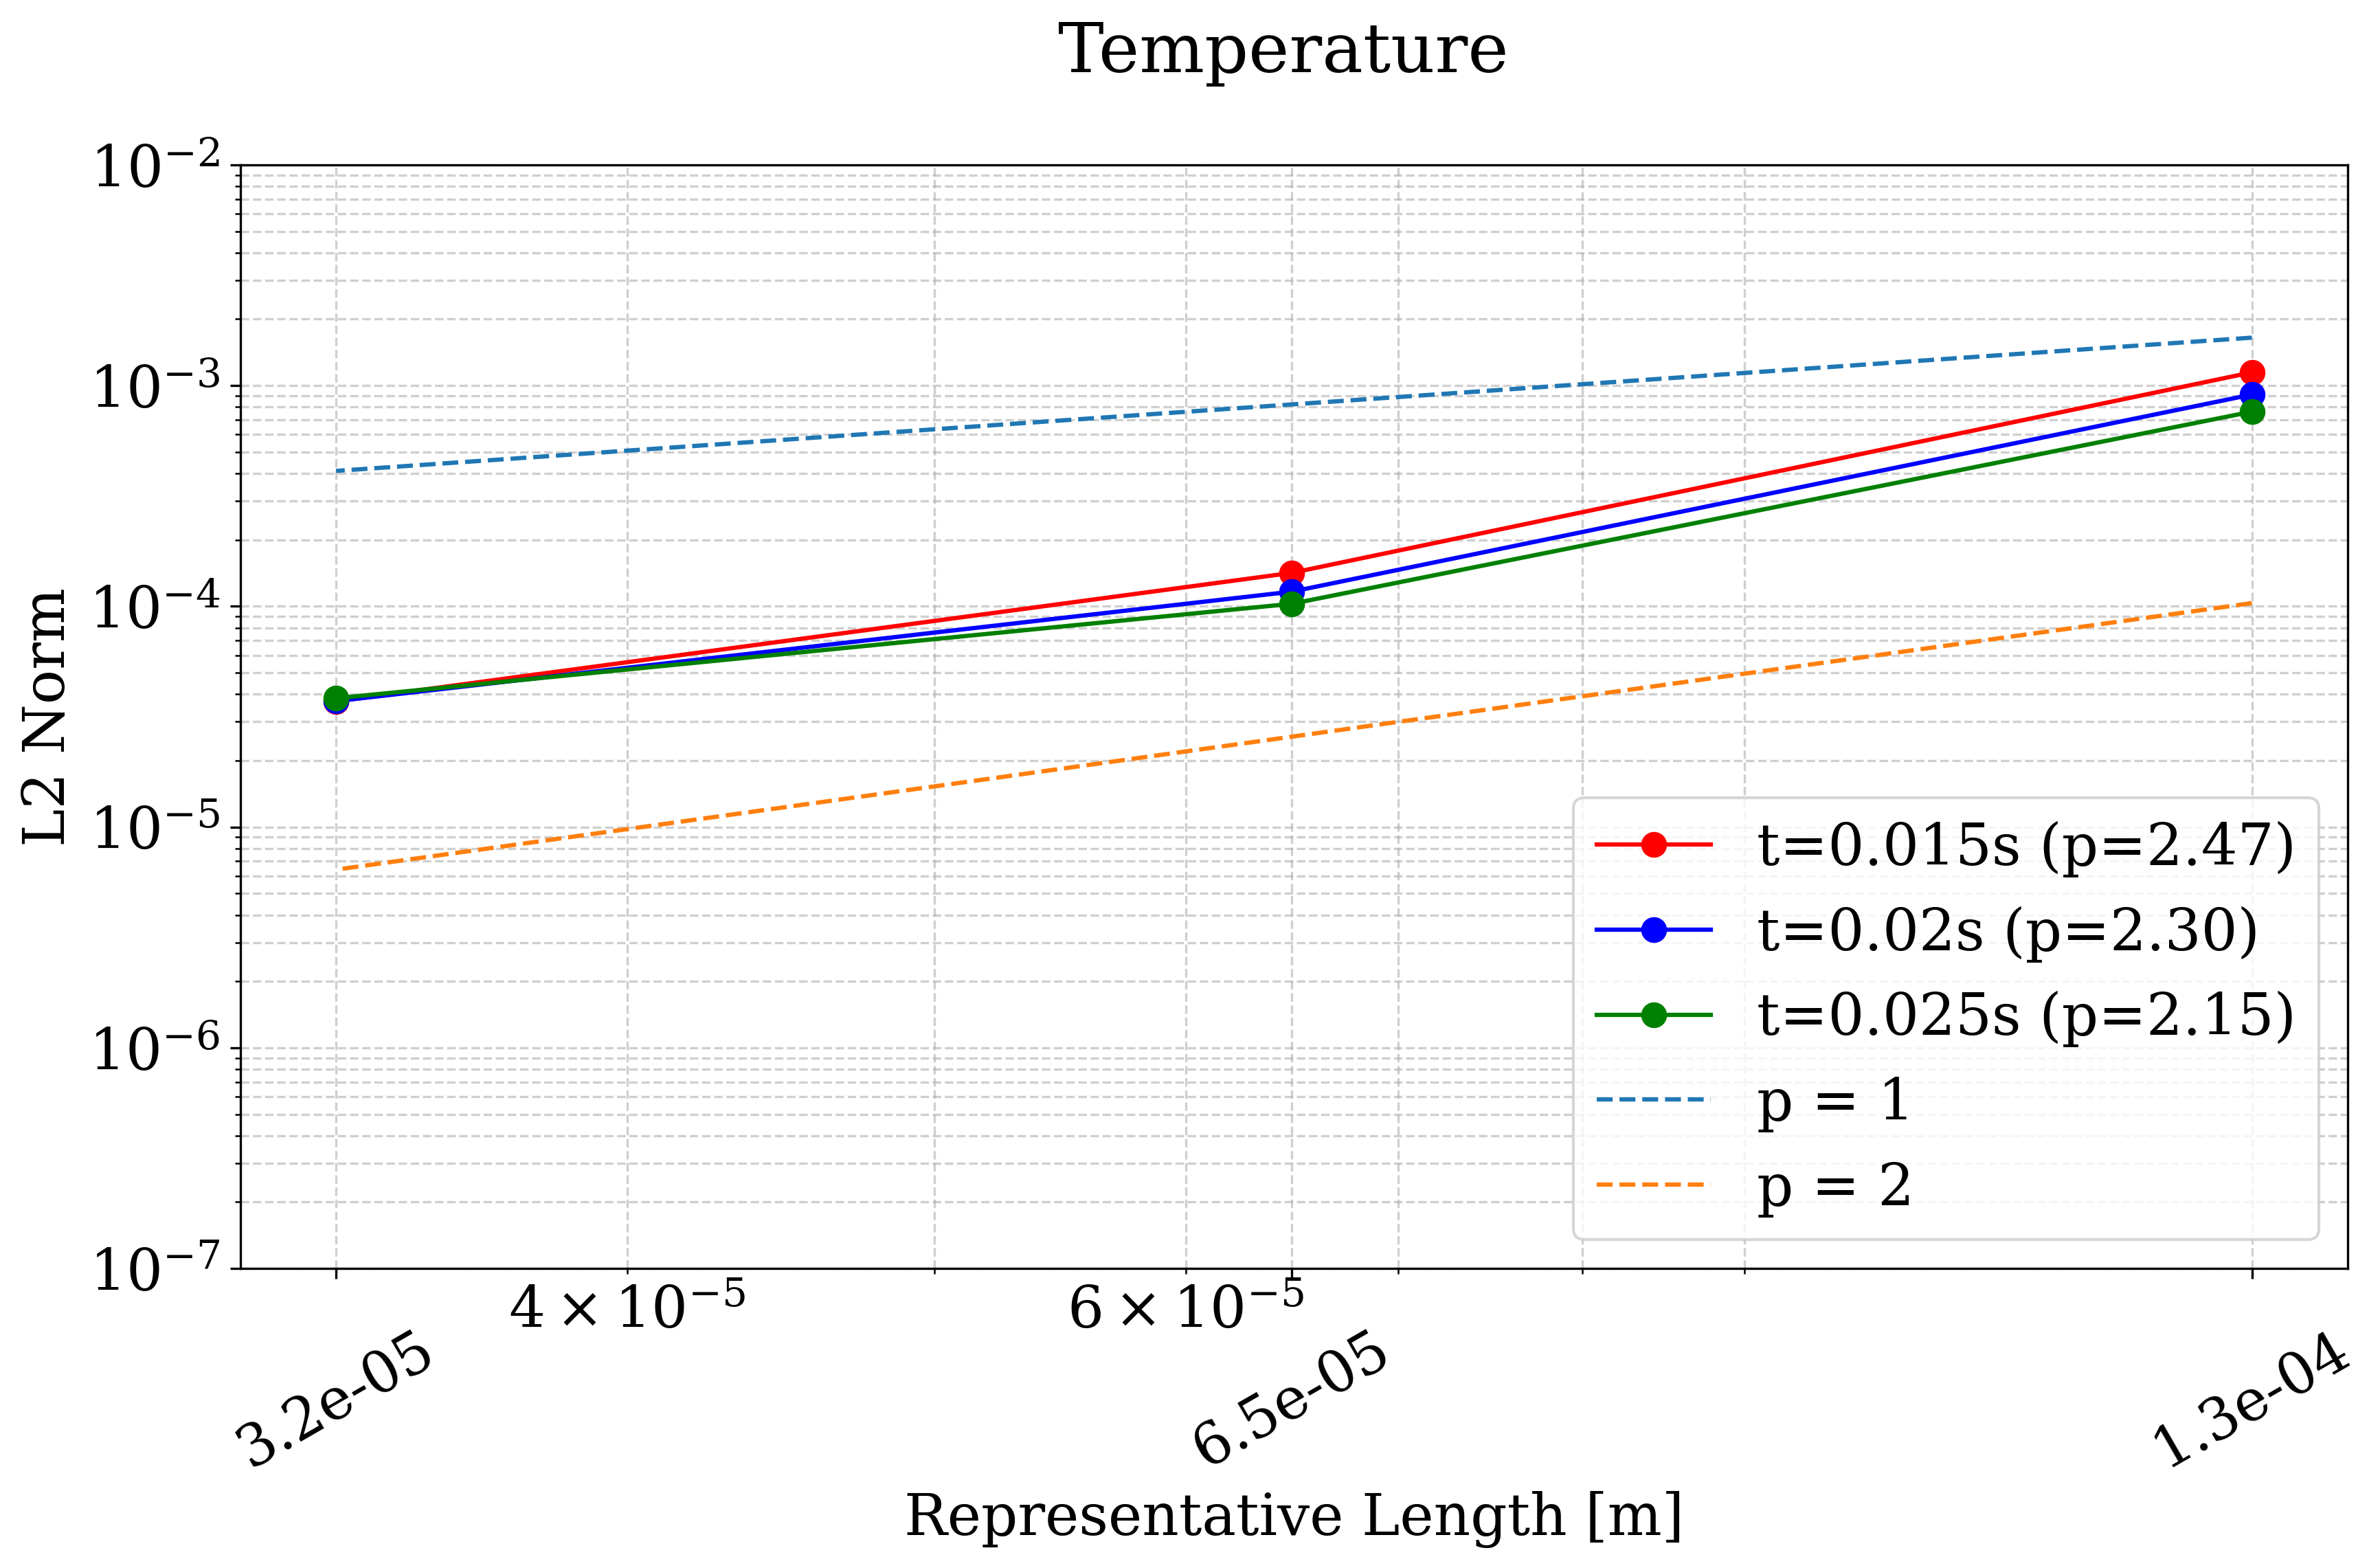
\includegraphics[width=1.0\linewidth]{figures/code_verification/interface/T_L2Norm_Observed_p_th2.png}
    \caption{Thermal diffusion model temperature $L_2$ error by representative cell length at three times.}
    \label{fig:transientDiffusionConvergence}
\end{figure}
The error decreases consistently with mesh refinement, yielding observed orders of convergence of $p=2.47$ at $t=0.015$~s, $p=2.30$ at $t=0.020$~s, and $p=2.15$ at $t=0.025$~s, showing near second-order spatial accuracy. Larger errors occur at earlier times due to stronger thermal gradients, while later times exhibit reduced error magnitudes as the solution becomes increasingly diffused. These results demonstrate that the solver accurately captures transient thermal diffusion behavior and correctly transfers the imposed solid temperature response across the fluid-solid interface under transient conditions.

\subsection{Solution Verification} 
Solution verification results are presented to quantify numerical error arising from spatial and temporal discretization, as well as solver convergence. The analysis focuses on the impact of mesh resolution, time step size, and solver tolerance on the predicted temperature response. The following studies evaluate convergence behavior and discretization error for both steady-state and transient models, building the accuracy and reliability of the coupled fluid-thermal solution.

\subsubsection{Steady-State Coupled Pipe}
Following independent verification of the fluid and solid governing equations, a fully coupled conjugate heat transfer (CHT) configuration is considered to assess the combined system behavior. The discretization error is evaluated through systematic mesh refinement under steady-state conditions. Figure~\ref{fig:scatterTemp} shows the radial temperature distribution within the thermally developing region, located 14 mm downstream of the start of heating. The highest temperatures occur near the wall where heat is introduced, while lower temperatures are near the centerline due to the developing thermal boundary layer. As mesh resolution increases, the temperature field becomes smoother and more consistent.

\begin{figure}[htbp]
  \centering
  \begin{subfigure}[b]{0.5\textwidth}
    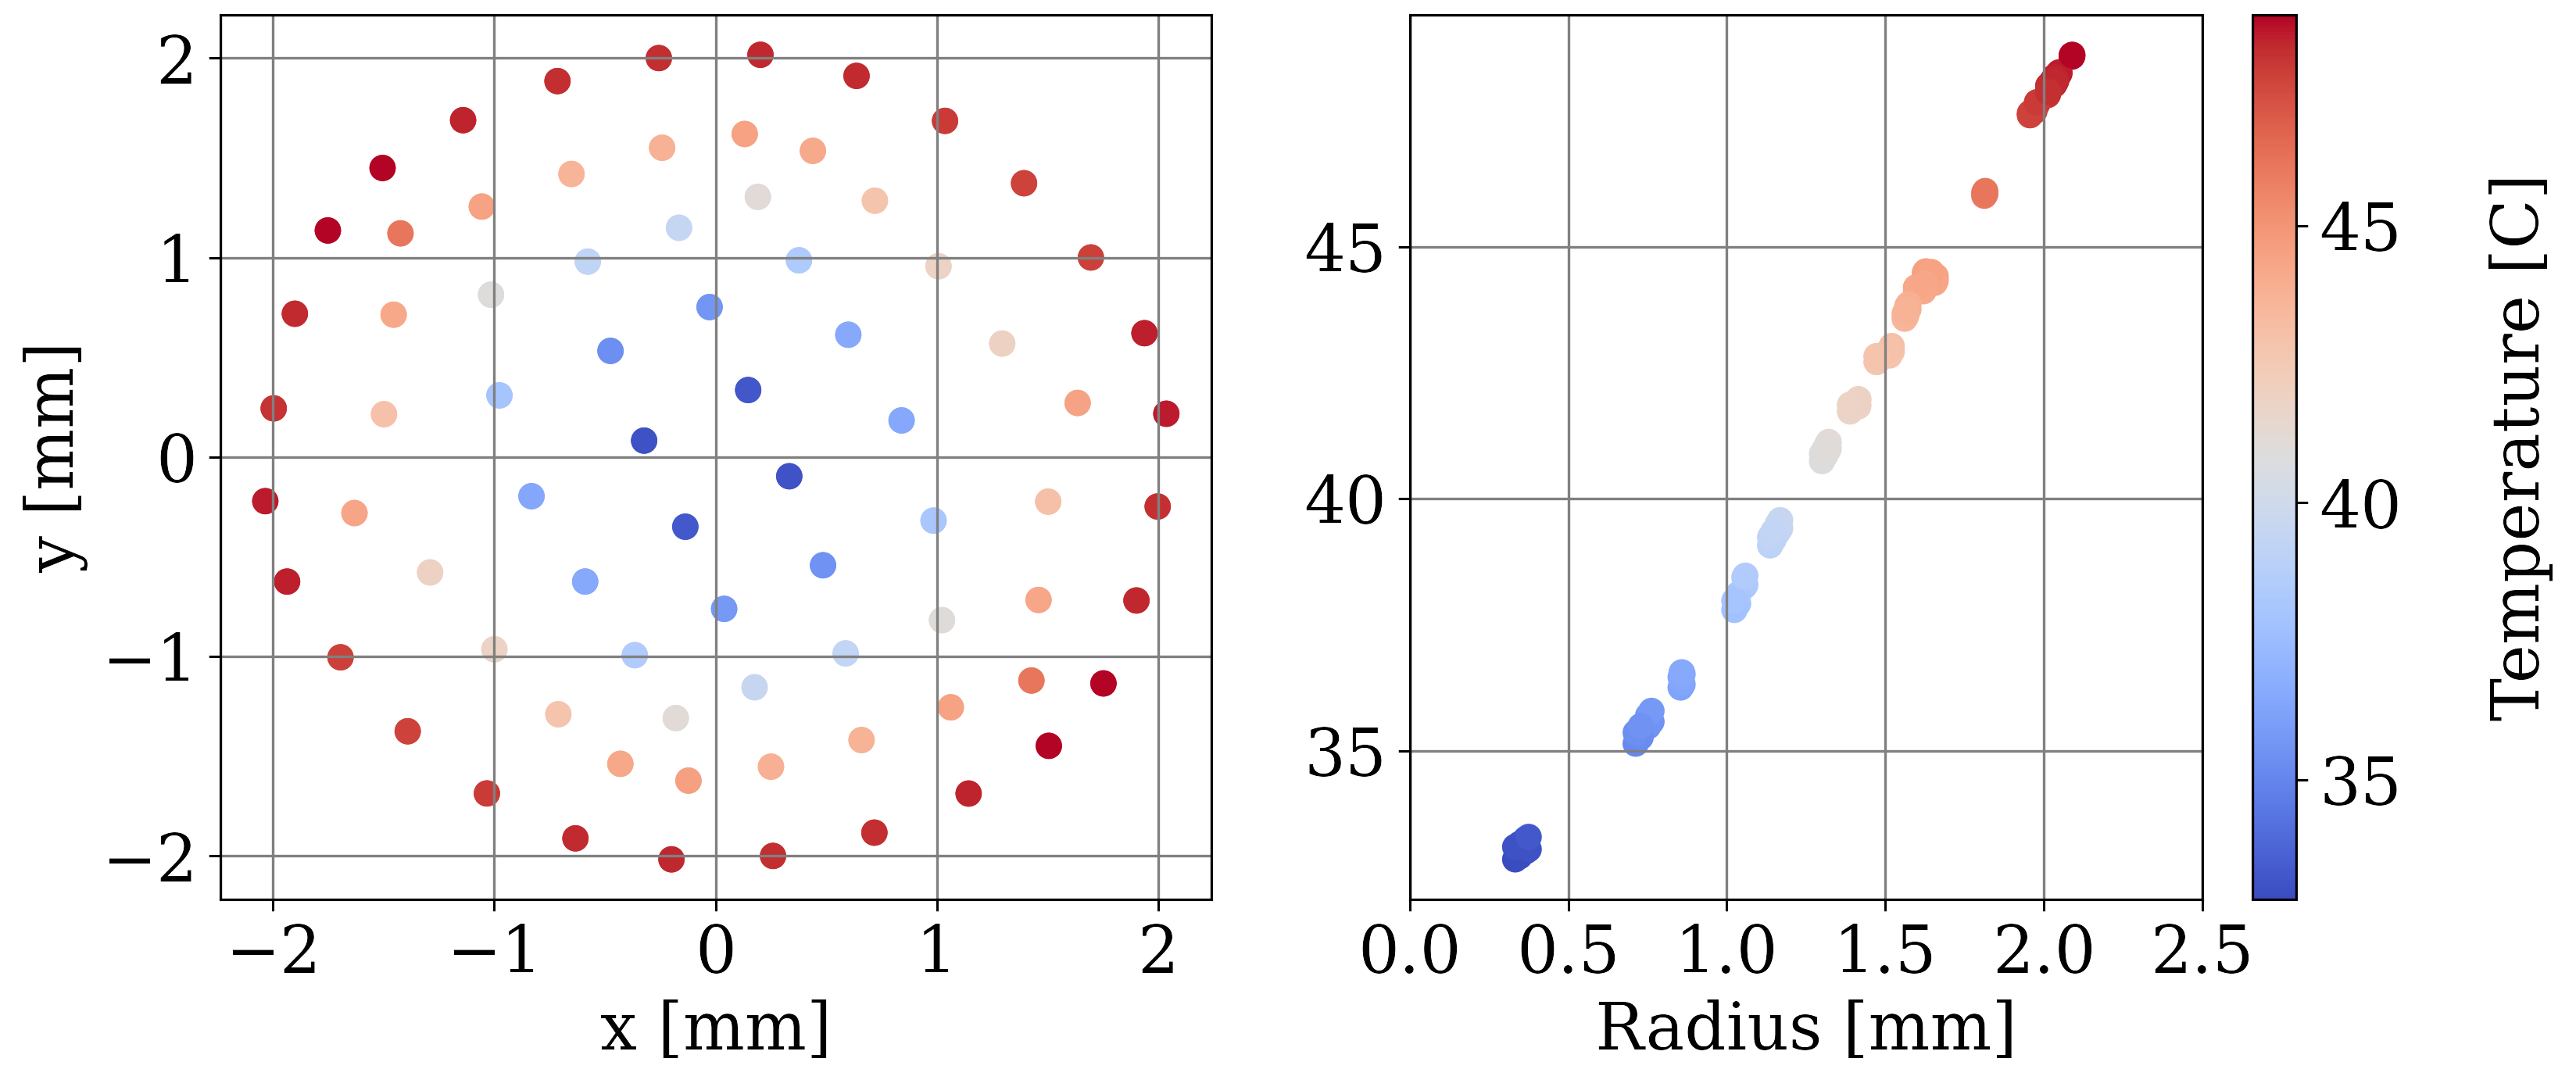
\includegraphics[width=\textwidth]{figures/code_verification/graetz/T_scatter_radial_z30mm_M0.png}
    \caption{Coarse mesh.}
    \label{fig:sub1}
  \end{subfigure}
  \hfill
  \begin{subfigure}[b]{0.5\textwidth}
    \includegraphics[width=\textwidth]{figures/code_verification/graetz/T_scatter_radial_z30mm_m1.png}
    \caption{Medium mesh.}
    \label{fig:sub2}
  \end{subfigure}
  \hfill
  \begin{subfigure}[b]{0.5\textwidth}
    \includegraphics[width=\textwidth]{figures/code_verification/graetz/T_scatter_radial_z30mm_m2.png}
    \caption{Fine mesh.}
    \label{fig:sub3}
  \end{subfigure}
  \caption{Radial temperature distribution within the thermally developing region.}
  \label{fig:scatterTemp}
\end{figure}

To quantify convergence, the bulk fluid temperature was evaluated downstream of the thermal development region at 30~mm and compared across mesh resolutions using an extrapolated solution obtained from the \texttt{StREEQ} method. Figure~\ref{fig:tempErrs_mesh} shows the relative error as a function of representative cell size on a log-log scale. The error decreases consistently with refinement, resulting in an observed order of convergence of $p = 1.90$, which is consistent with near second-order spatial accuracy. These results demonstrate that the coupled solver exhibits consistent convergence behavior and accurately captures the thermally developing flow.

\begin{figure}[htbp!]
    \centering
    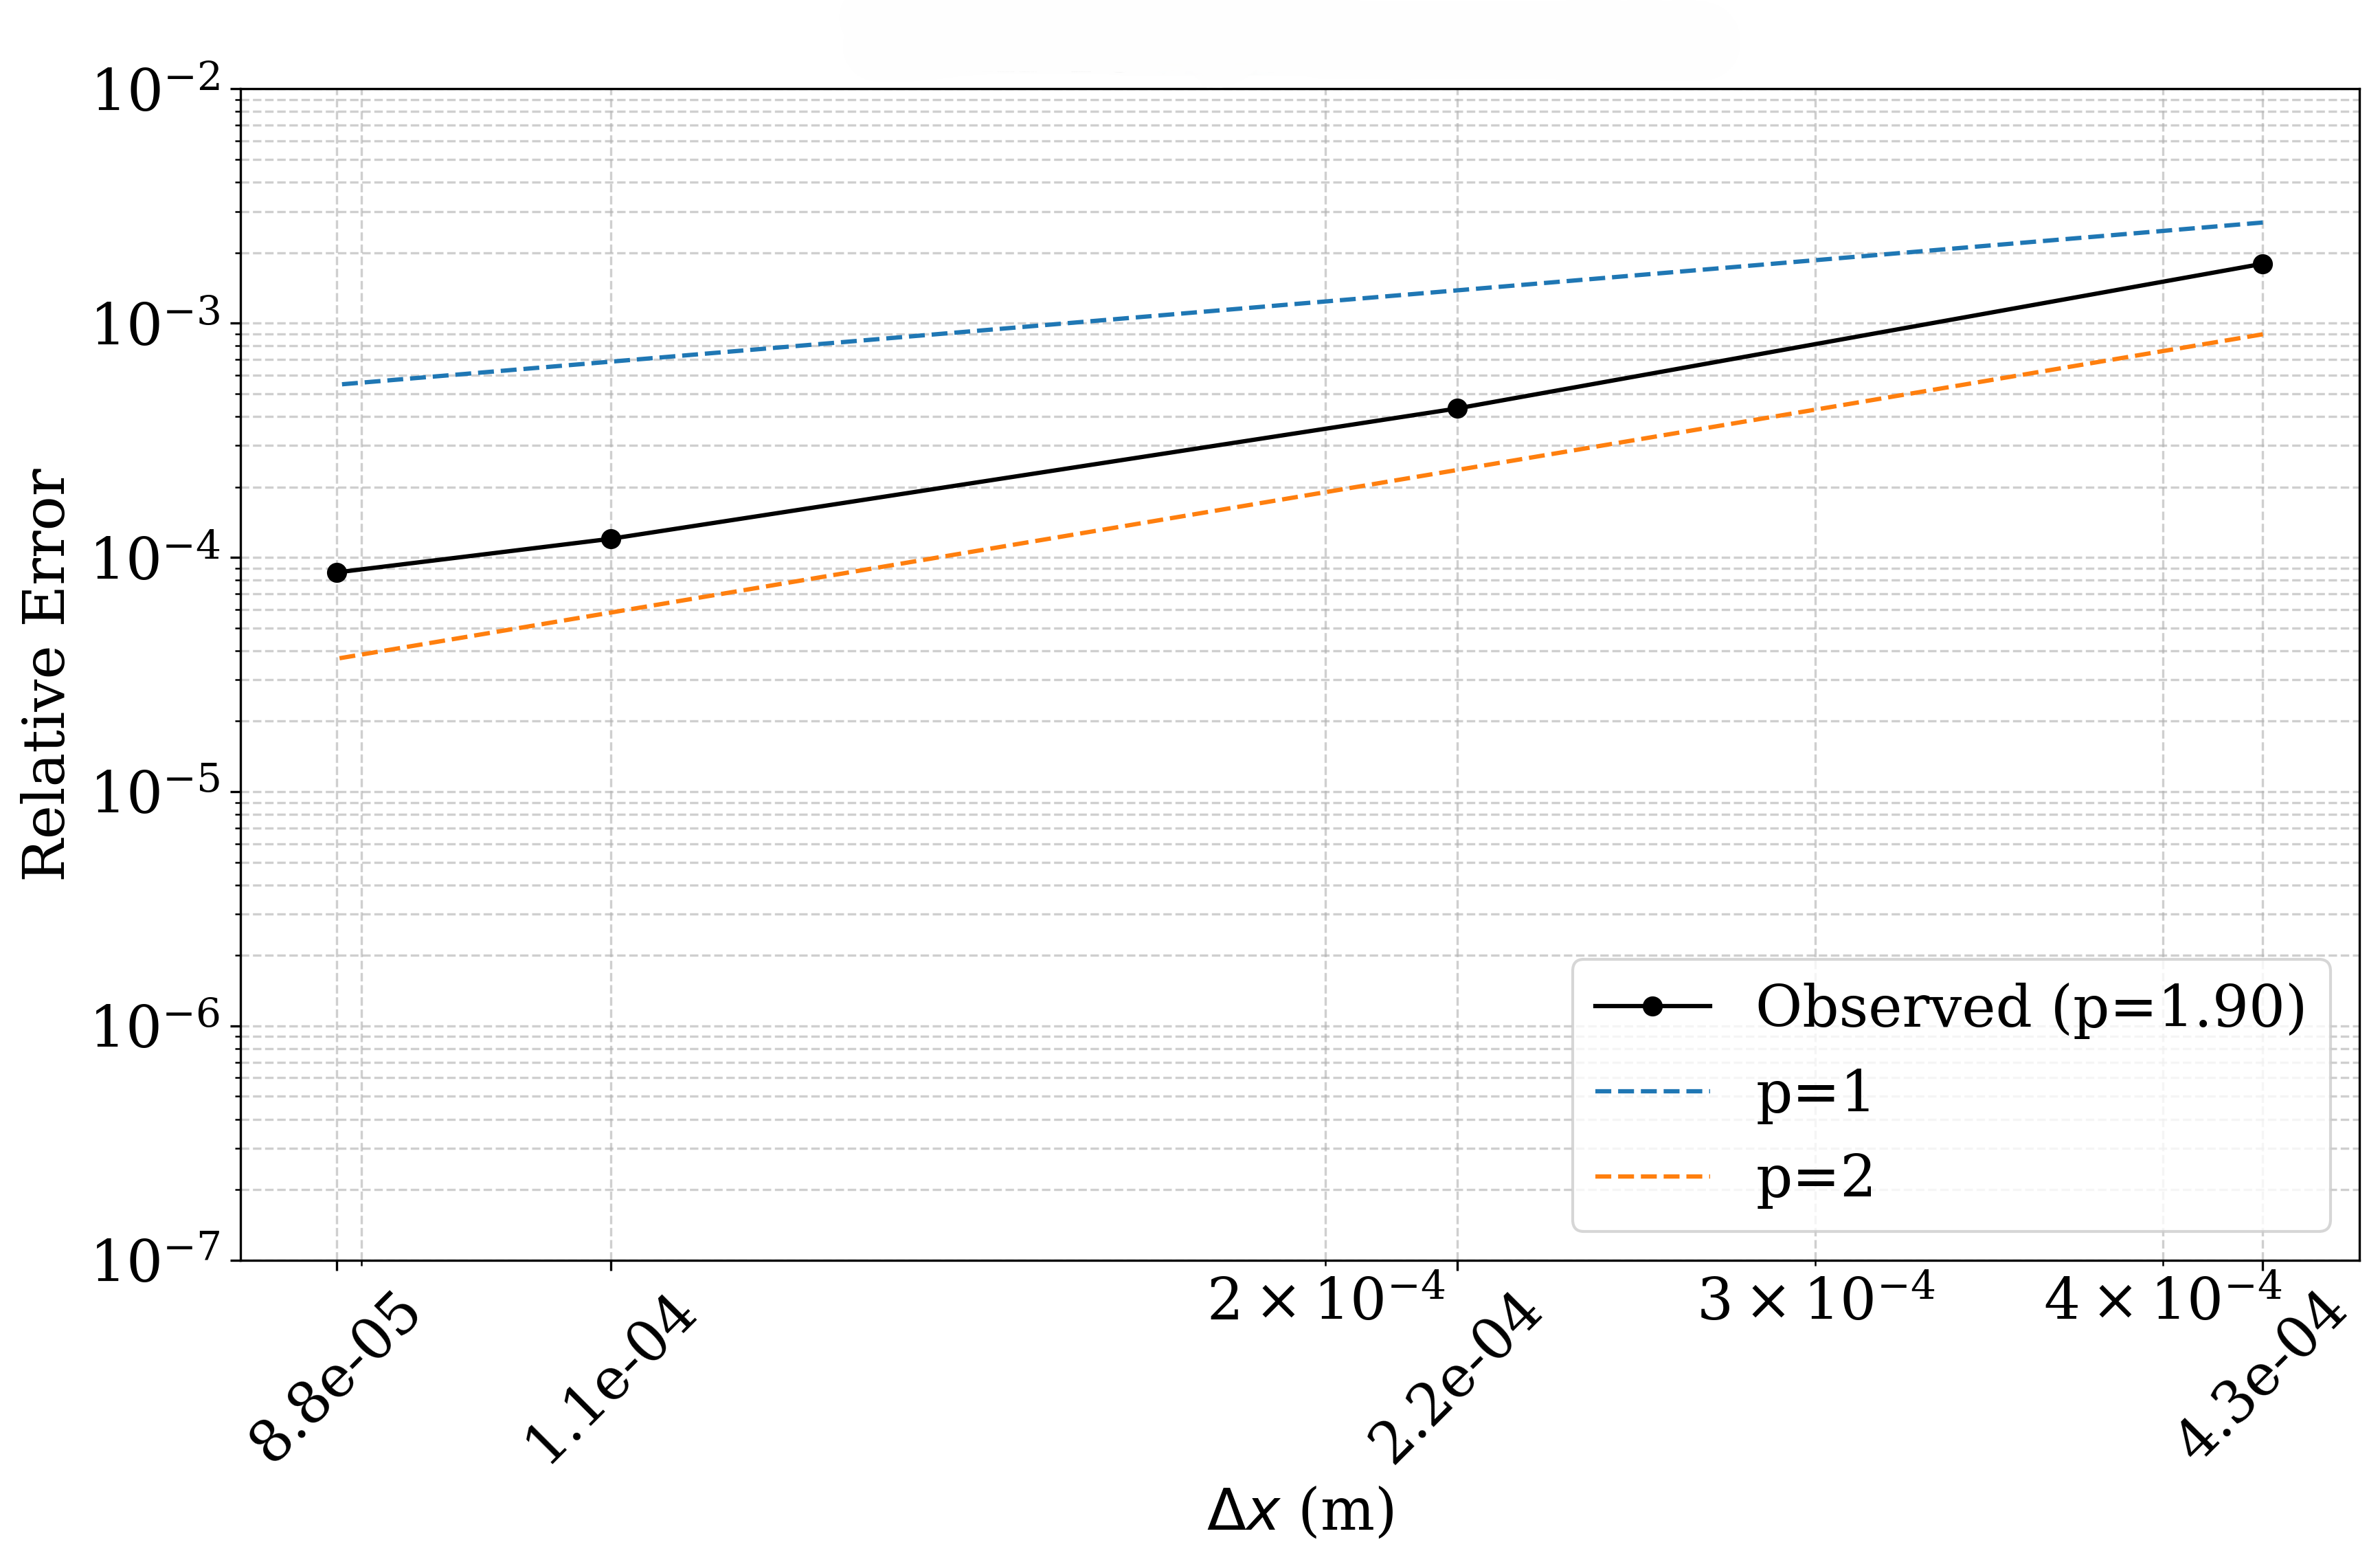
\includegraphics[width=1.0 \linewidth]{figures/code_verification/graetz/relative_err_observedP_mesh_Tbulk.png}
    \caption{Relative error in bulk temperature versus representative mesh cell size, with observed order of convergence $p = 1.90$.}
    \label{fig:tempErrs_mesh}
\end{figure}


\subsubsection{Transient Simplified EDDS}
To evaluate the coupled effects of spatial and temporal discretization, a co-refinement study was performed in which seven mesh levels (M1–M7) were paired with progressively refined time steps (T1–T7). This approach assesses how discretization errors evolve in a transient, coupled fluid-thermal system. Figure~\ref{fig:meshTimestep} shows the relative error estimated using the \texttt{StREEQ} model (Eq.~\ref{eq:streeq_model_p2}) across all mesh-timestep combinations. The error ranges from $\mathcal{O}(10^{-2})$ for coarse configurations to $\mathcal{O}(10^{-4})$ for the finest cases. A trend is observed in which error decreases with both mesh refinement and timestep reduction, indicating that spatial and temporal discretization contribute jointly to the numerical error. The relative errors show a nearly linear gradient across the mesh-timestep space, suggesting a balanced influence of spatial and temporal resolution. This behavior highlights the coupled nature of discretization error in transient simulations, where neither spatial nor temporal refinement alone is sufficient to achieve convergence.
% The coarsest combinations show substantial error accumulation after 5 seconds, while finer resolutions converge toward a consistent solution. The combination of M3 and T3 case shows less than 0.1\% error, supporting its use in downstream analysis.

\begin{figure}[htbp!]
    \centering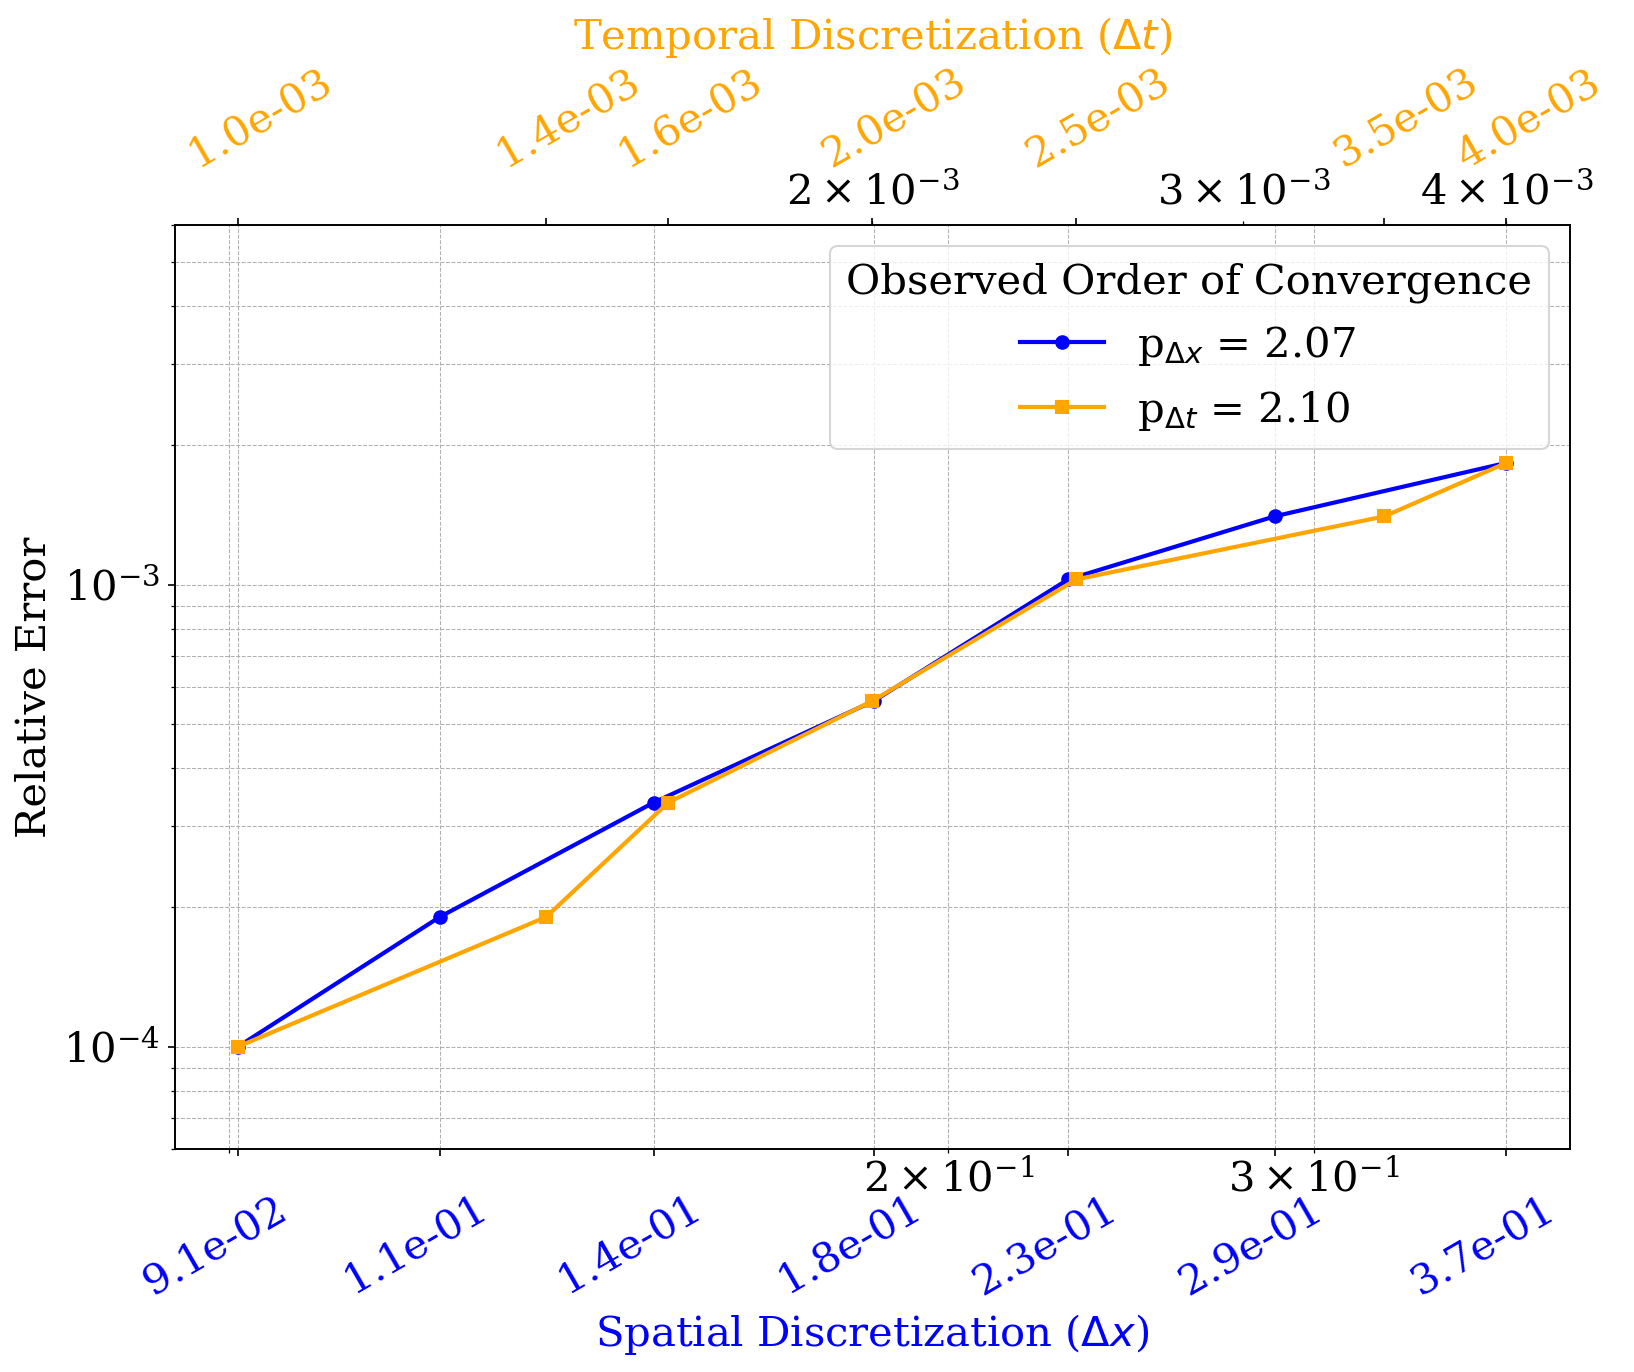
\includegraphics[width=1.0 \linewidth]{figures/solution_verification/relative_err_observedP_meshANDtimestep.png}
    \caption{Relative error across mesh-timestep combinations from the co-refinement study.}
    \label{fig:meshTimestep}
\end{figure}


\subsubsection{Solver Tolerance Study}
This study is conducted for the transient simplified EDDS configuration, where iterative solver convergence can influence the time-dependent thermal response.
To assess the impact of linear solver convergence criteria on the predicted thermal response, a solver tolerance study was conducted using mesh M3 and time step 0.005~s. Six convergence tolerances ranging from $10^{-3}$ to $10^{-8}$ were evaluated. The coarsest tolerance ($10^{-3}$) underpredicts the temperature response throughout the simulation. As the tolerance is tightened, the solutions converge toward a consistent response. The results for $10^{-7}$ and $10^{-8}$ are visually indistinguishable, indicating that solver-induced numerical error is negligible at these tolerances. Relative error was computed using the most stringent tolerance ($10^{-8}$) as the reference solution. The error decreases from $\mathcal{O}(10^{-1})$ at $10^{-3}$ to $0$ at $10^{-8}$. A tolerance of $10^{-6}$ yields a relative error below $0.0125\%$, indicating sufficient solver accuracy for this problem.

\subsubsection{Decoupled Resolution Analysis} 
To assess the impact of independently refining spatial and temporal discretization, mesh-only and timestep-only studies were performed and compared against the co-refinement results. Figure~\ref{fig:decoupledConvergence} shows that while error decreases with refinement in both cases, the observed convergence rates ($p \approx 1.06$) are significantly lower than the expected second-order behavior. This indicates that unresolved discretization error from the fixed parameter (time or space) influences the solution.

\begin{figure}[htbp!]
    \centering
    \begin{subfigure}[b]{\linewidth}
        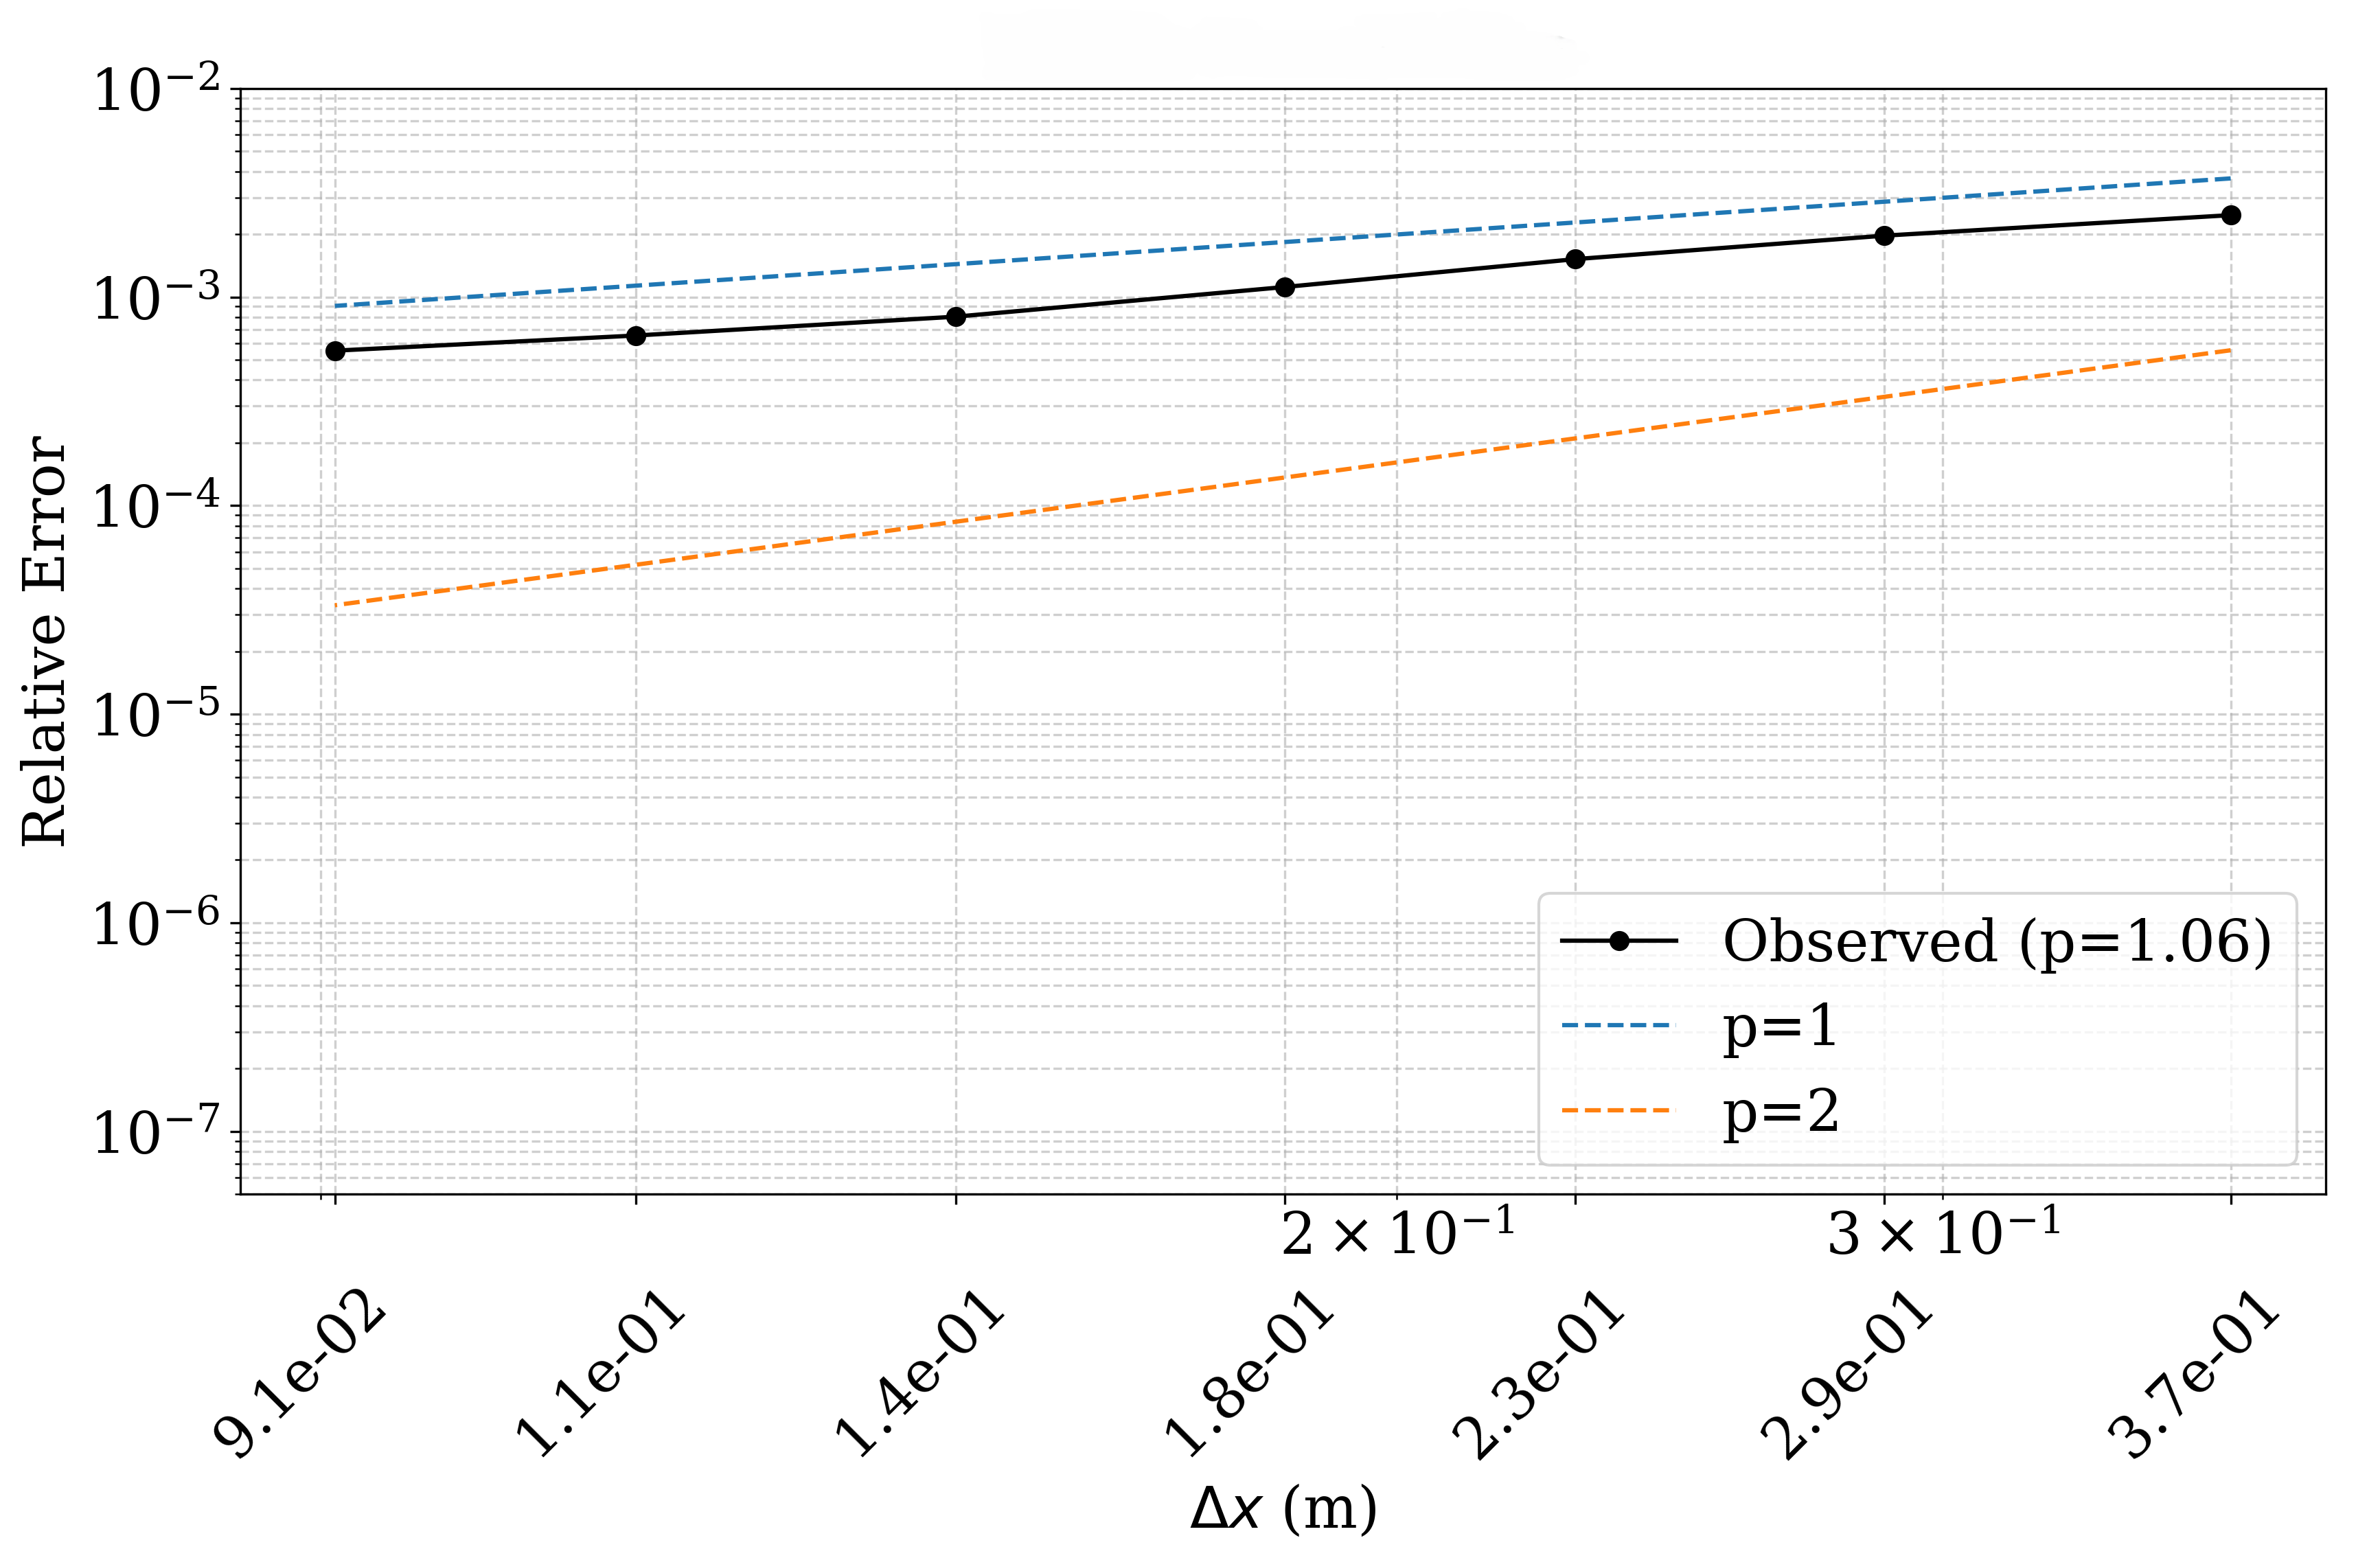
\includegraphics[width=\linewidth]{figures/solution_verification/relative_err_observedP_mesh.png}
        \caption{Mesh-only refinement (fixed timestep).}
    \end{subfigure}
    \vspace{0.5em}
    \begin{subfigure}[b]{\linewidth}
        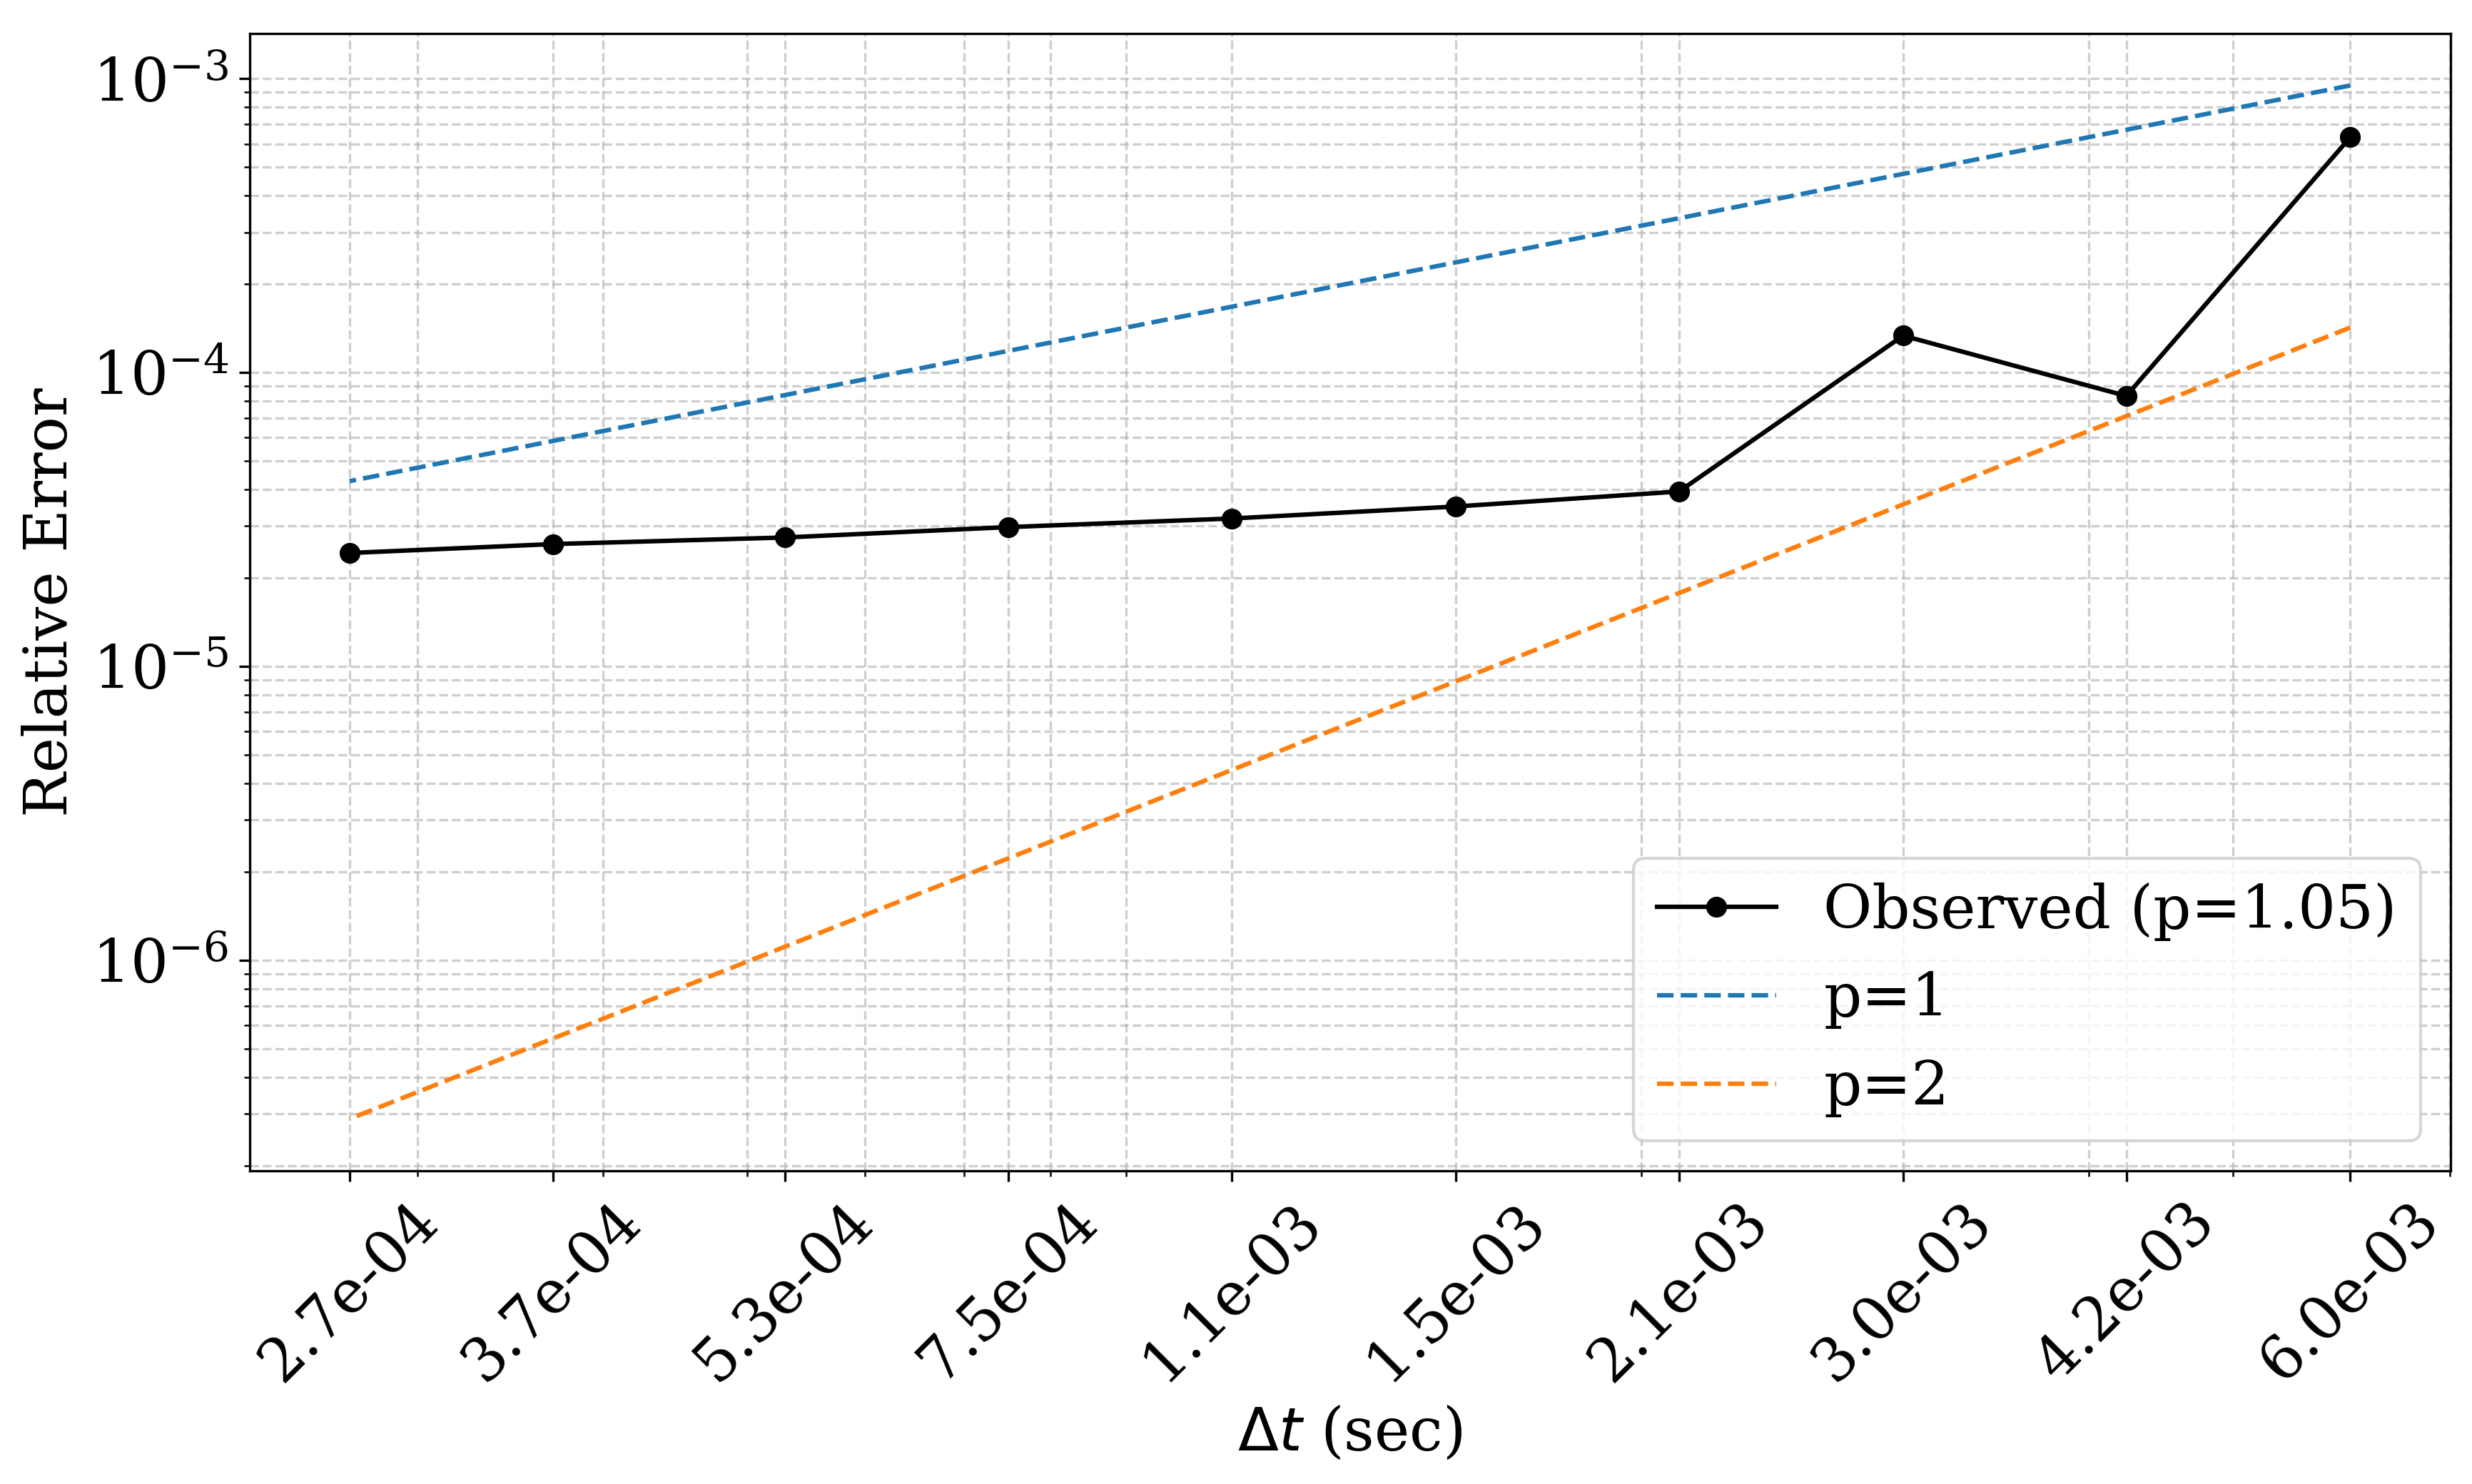
\includegraphics[width=\linewidth]{figures/solution_verification/relative_err_observedP_Tavg_z0.03_t5.png}
        \caption{Timestep-only refinement (fixed mesh).}
    \end{subfigure}
    \caption{Observed convergence behavior for independent mesh and timestep refinement studies. Both cases exhibit reduced convergence rates ($p \approx 1.06$), indicating the influence of unresolved discretization error from the fixed parameter.}
    \label{fig:decoupledConvergence}
\end{figure}

Comparison with the co-refinement results (Figure~\ref{fig:meshTimestepAll}) shows that independent refinement can under- or overestimate numerical error. In contrast, co-refinement captures the coupled influence of spatial and temporal discretization, providing a more reliable assessment of convergence behavior. These results demonstrate that independent refinement is insufficient for accurately characterizing discretization error in transient conjugate heat transfer simulations.

\begin{figure}[htbp!]
    \centering
    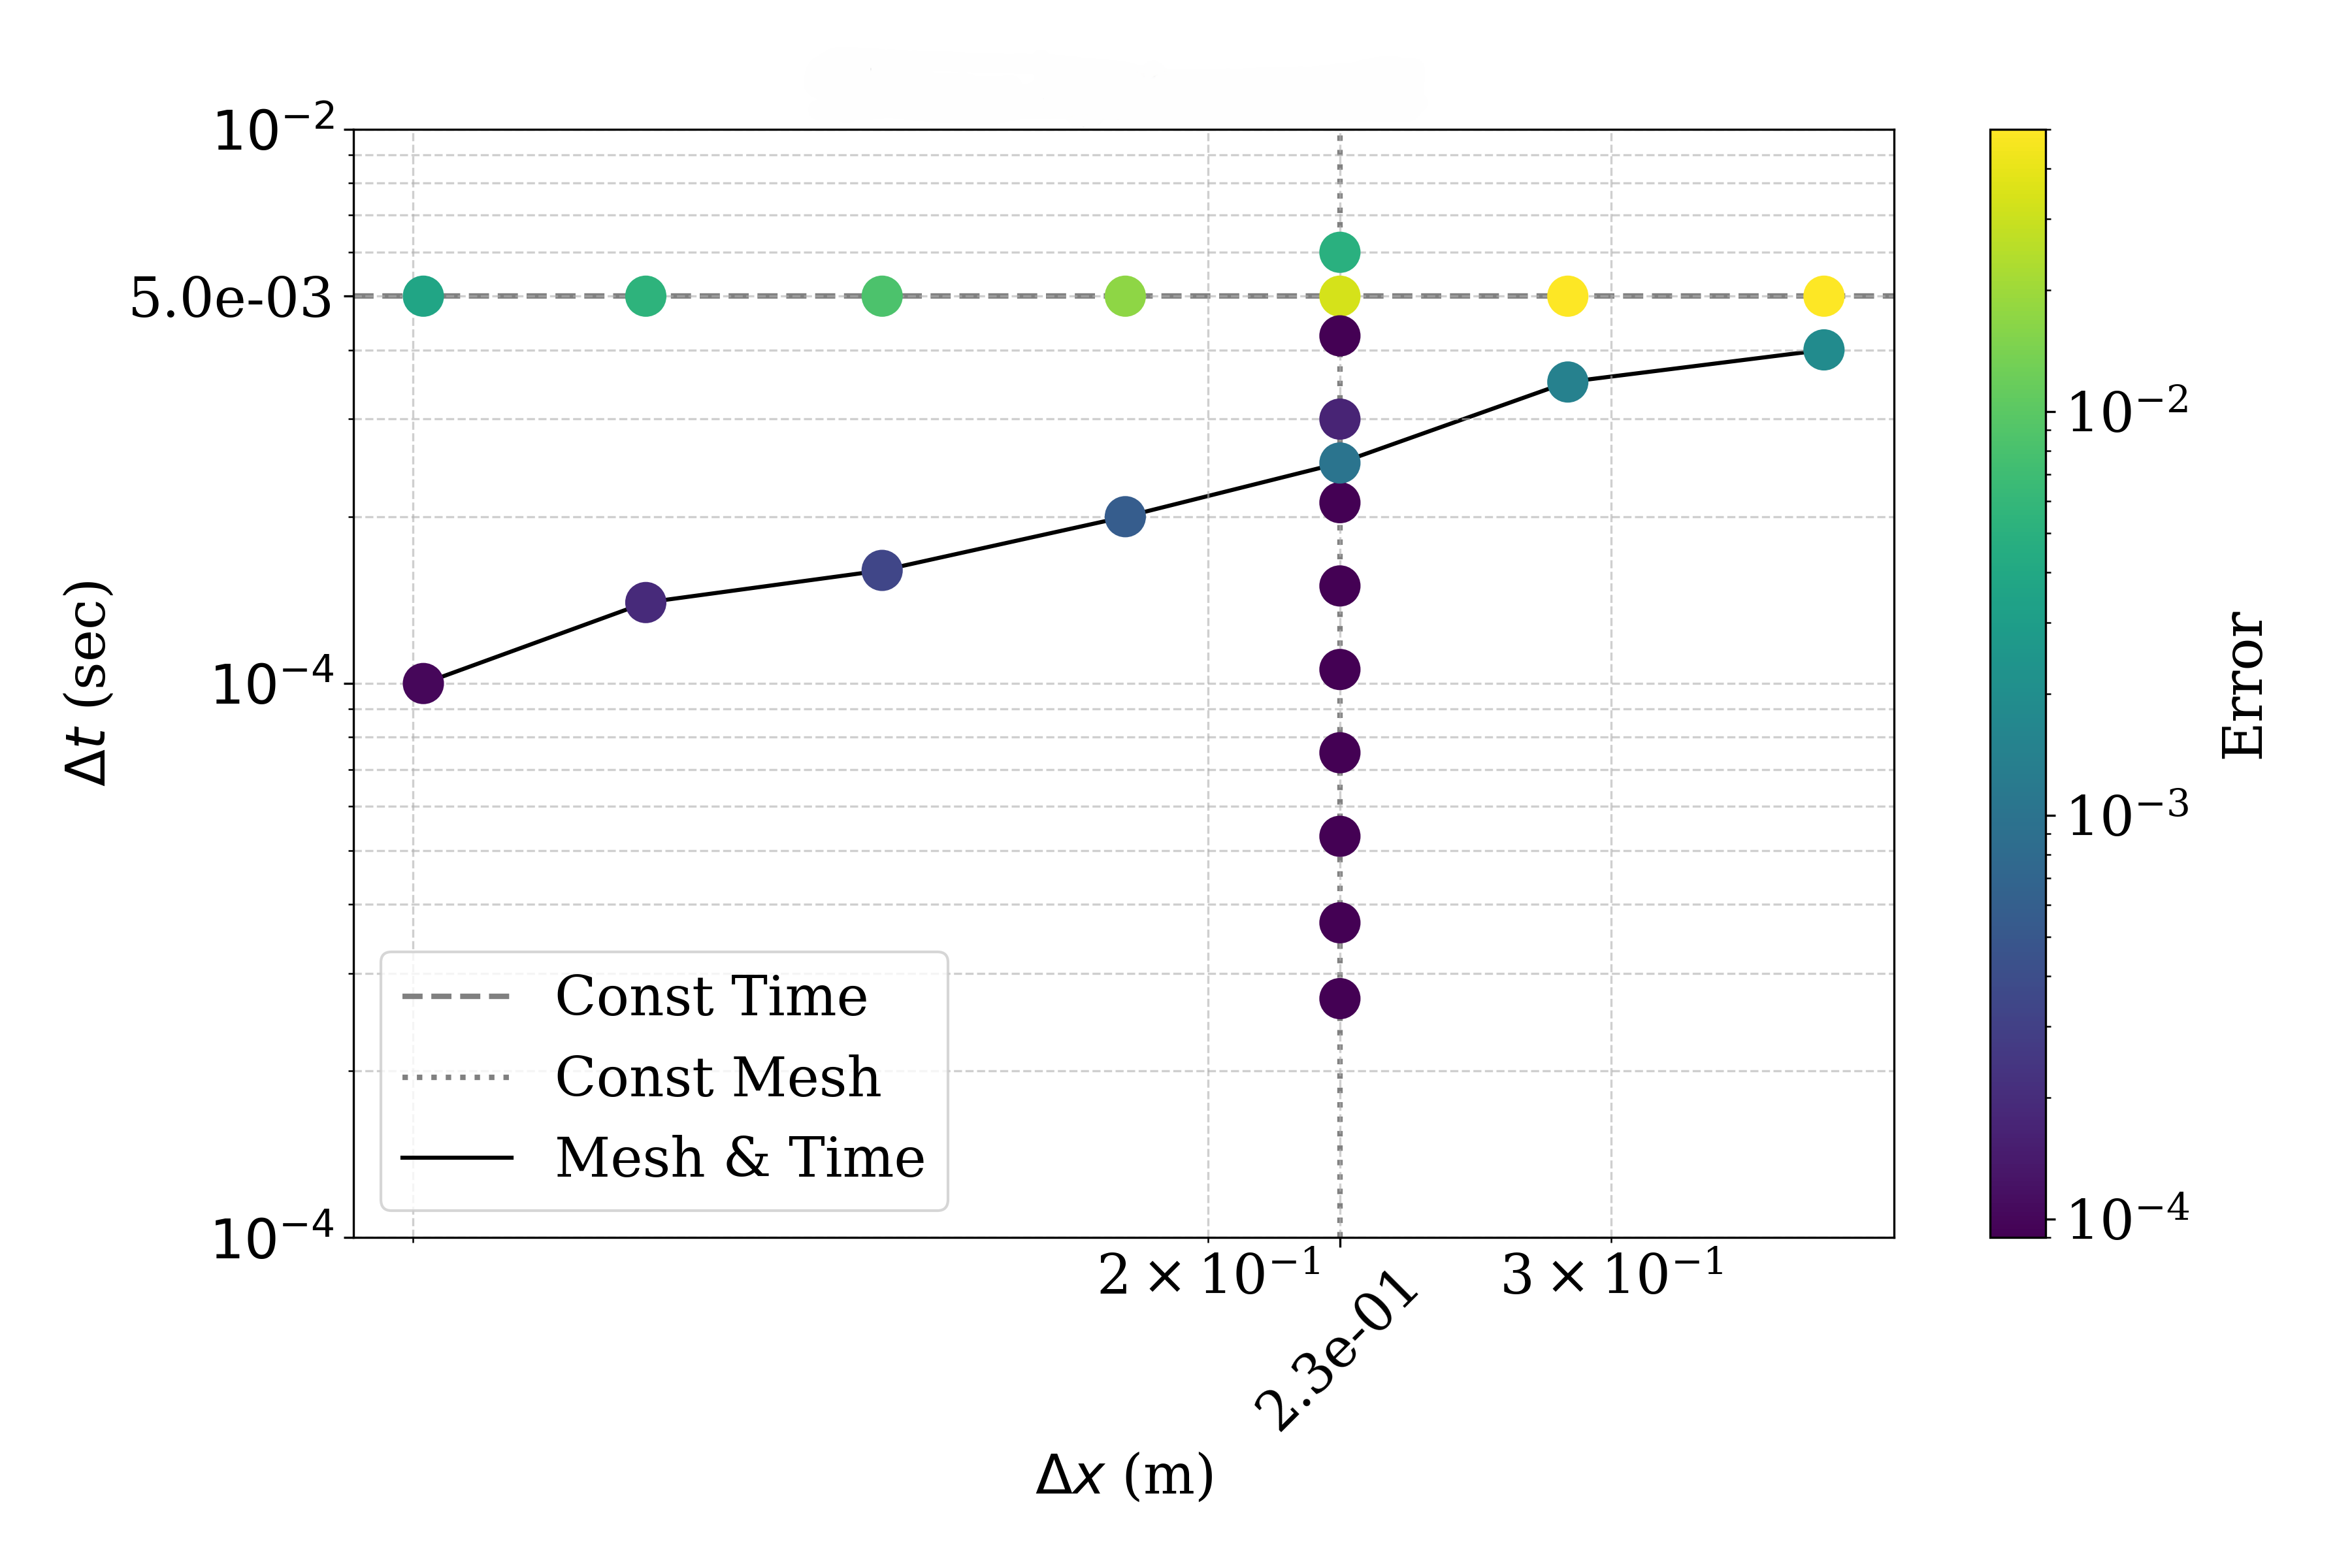
\includegraphics[width=\linewidth]{figures/solution_verification/streeq_scatter_error_Temperature_meshTime_all.png}
    \caption{Relative error across mesh and timestep combinations, including co-refined and independently refined cases.}
    \label{fig:meshTimestepAll}
\end{figure}


\subsection{Interface Energy Consistency}
To ensure that the coupled conjugate heat transfer satisfies heat-flux continuity, an additional analysis was performed on the simplified EDDS model at the fluid-solid interface with the interface discretization refining consistently with the global mesh. It is expected that the heat flux leaving the solid must equal the heat flux entering the fluid, such that $Q_{\text{solid}} + Q_{\text{fluid}} \approx 0$. The interface imbalance was defined as
\begin{equation}
\epsilon_{\text{iface}} = |Q_{\text{solid}} + Q_{\text{fluid}}|.
\label{eq:interface_imbalance}
\end{equation}
The interface energy imbalance, normalized by the applied heat source, remained on the order of $\mathcal{O}(10^{-4})$ across all mesh resolutions and did not exhibit a clear dependence on mesh refinement. Multiple competing errors, which include interface interpolation, solver tolerances, and velocity-temperature coupling, prevent the interface imbalance from decreasing with mesh refinement because the interface flux depends on temperature gradients that are highly sensitive to local discretization.

% The interface energy imbalance normalized by the applied heat source remained on the order of  $\mathcal{O}(10^{-4})$ and did not exhibit a clear dependence on mesh resolution. This indicates that the imbalance is not governed solely by spatial discretization error. This corresponds to 0.01\% of the applied heat source. Although this metric is not used as a primary discretization-error estimate, its magnitude indicates that the interface energy mismatch is negligible relative to the imposed thermal loading and is unlikely to affect the observed convergence trends in the quantities of interest. 

% This analysis was performed for both the steady-state coupled pipe model and the radial conduction model . For the radial conduction case, the interface imbalance was observed to be on the order of $\mathcal{O}(10^{-6})$. For the coupled steady-state configuration, the imbalance was on the order of $\mathcal{O}(10^{-5})$ across all mesh resolutions. For the transient simplified EDDS model the imbalance was observed to be on the order of $\mathcal{O}(10^{-4})$ . In the radial conduction case, the interface imbalance decreased with mesh refinement. In contrast, the coupled configuration did not exhibit a clear monotonic reduction in imbalance with increasing mesh resolution, although the magnitude remained small for all meshes considered.


% To ensure that the coupled conjugate heat transfer solution is physically consistent, an additional analysis was performed at the fluid–solid interface. While prior code verification studies assessed the fluid and solid physics in isolation, the coupled configuration introduces the possibility that discretization at the interface may lead to non-physical energy imbalance, even under mesh refinement. For a physically consistent solution, the heat flux leaving the solid must equal the heat flux entering the fluid at the interface, $Q_{solid} + Q_{fluid} \approx 0$. To assess this, the total heat flux on each side of the interface was computed and the interface imbalance was defined as: $\epsilon_{iface} = |Q_{solid} + Q_{fluid}|$. For the radial conduction case the difference in heat flux are on the order of magnitude of $\mathcal{O}(10^{-6})$ and for the coupled steady state case on the $\mathcal{O}(10^{-5})$. 

% Despite mesh refinement, the interface imbalance in the coupled configuration does not exhibit a clear monotonic reduction. This behavior is attributed to the presence of multiple competing error sources, including interpolation across the fluid–solid interface, solver convergence tolerances, and coupling between the velocity and temperature fields. Unlike the radial conduction case, where the error is dominated by spatial discretization, the coupled configuration introduces additional numerical errors that do not scale directly with mesh refinement. Furthermore, because the interface flux depends on temperature gradients, it is more sensitive to local discretization and interpolation errors than the primary solution variables. As a result, the interface imbalance approaches a plateau governed by solver and coupling errors rather than purely spatial resolution.

% Despite the absence of strict monotonic convergence, the magnitude of the interface imbalance remains small. This indicates that energy is well conserved across the interface and that the coupled solution is physically consistent for the purposes of this study.

\subsection{Computational Cost}
Computational cost was evaluated for the transient simplified EDDS configuration to assess the trade-off between numerical accuracy and resource requirements. Figure~\ref{fig:compCost} summarizes the cost across mesh and timestep combinations. The simulations for each of these combinations were conducted on an Intel Xeon Broadwell (BDW) E5-2695v4 at 2.1 GHz with 18 core CPU workstations. 

For the intermediate resolution case (M3 with $\Delta t = 0.0025$ s), the relative error is approximately $0.1\%$ with a computational cost of 24 minutes. Refinement to M4 with $\Delta t = 0.002$ s reduces the error to $0.055\%$, but increases computational cost to 47 minutes, corresponding to a 96\% increase in cost for a 45\% reduction in error. 

\begin{figure}[htbp!]
    \centering
    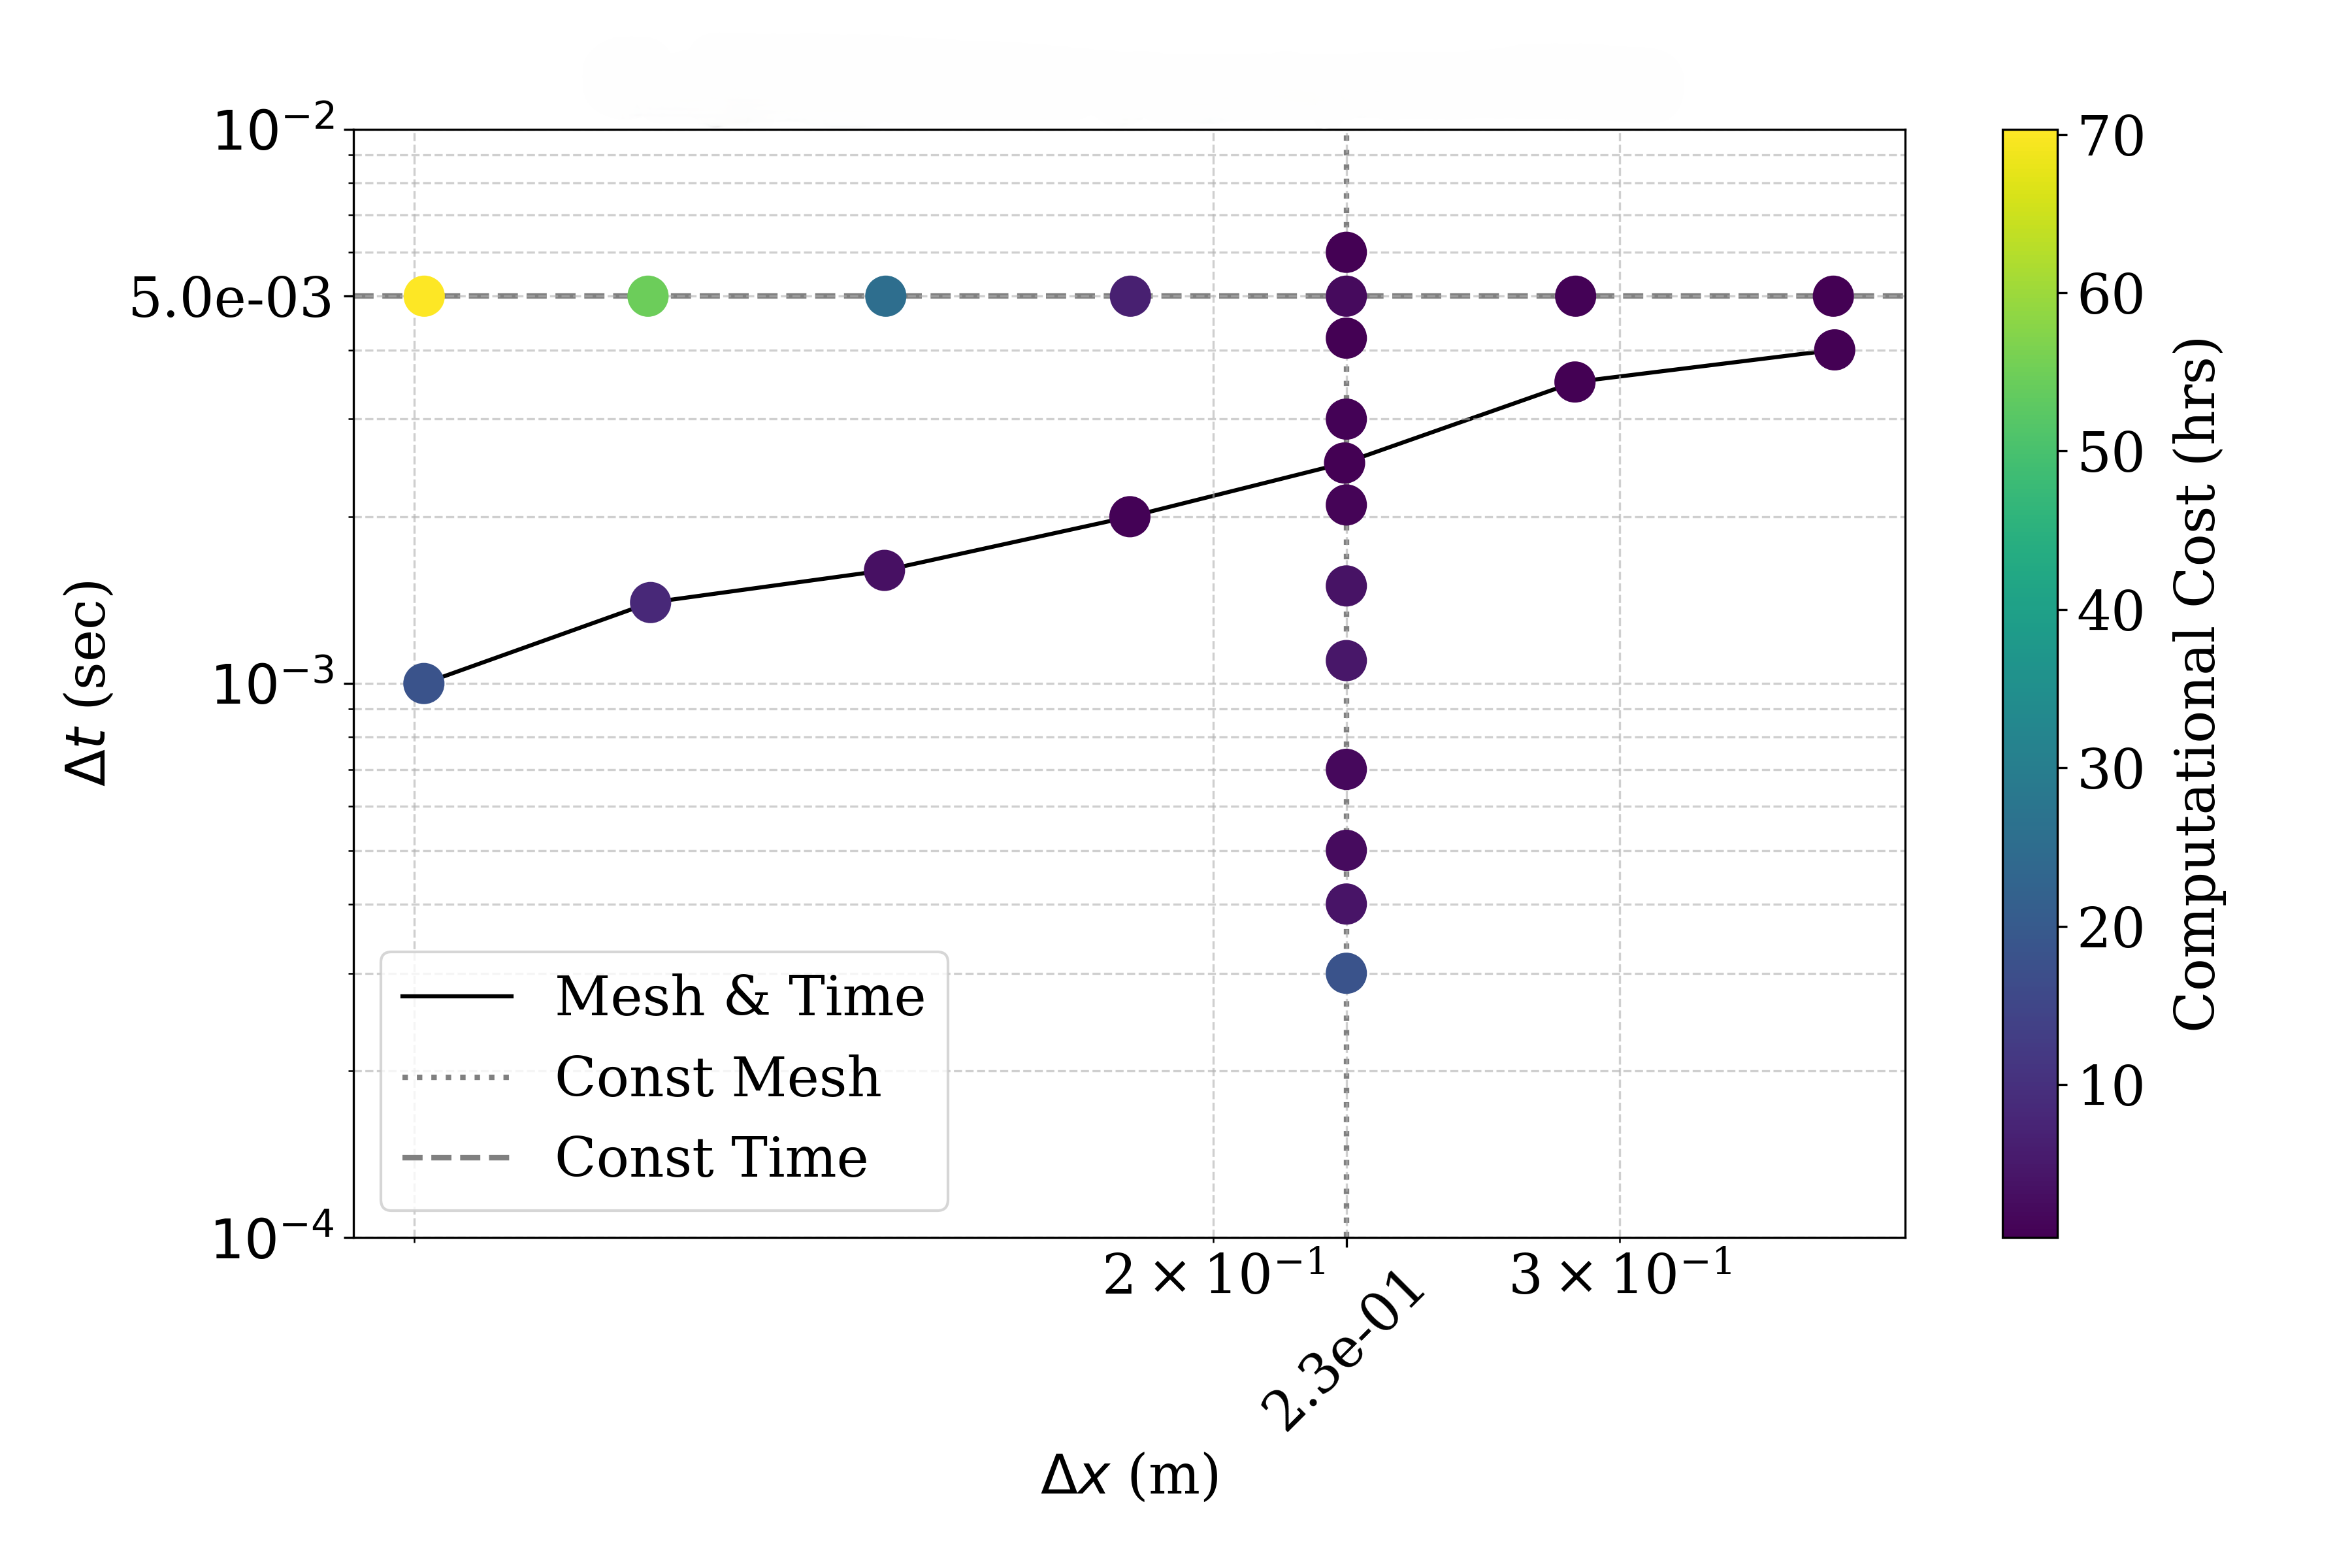
\includegraphics[width=1.0 \linewidth]{figures/solution_verification/scatter_dxdt_comCost_all.png}
    \caption{Computational Cost in hours across mesh, time step, and combined mesh time step studies. }
    \label{fig:compCost}
\end{figure}

These results demonstrate diminishing returns with increased resolution, where significant increases in computational cost yield comparatively small gains in accuracy. This trade-off highlights the importance of selecting discretization parameters that balance accuracy with computational efficiency, particularly in resource-constrained environments. Based on this analysis, the M3–T3 configuration provides a practical balance between accuracy and cost, and is selected for subsequent validation studies. This selection also supports reproducibility by enabling the study to be executed within accessible computational resources while maintaining sufficient numerical accuracy.
